\pagestyle{fancy}
\headheight 20pt
\lhead{Ph.D. Thesis --- T.~J. Parkin }
\rhead{McMaster - Physics \& Astronomy}
\chead{}
\lfoot{}
\cfoot{\thepage}
\rfoot{}
\renewcommand{\headrulewidth}{0.1pt}
\renewcommand{\footrulewidth}{0.1pt}

\chapter{Introduction} \label{chapter1} 

\thispagestyle{fancy} 
The night sky is full of stars, the moon and planets, galaxies and a variety of other galactic objects.  Historically, our perspective of these objects was limited to what we could see with our eyes or through an optical telescope, which covers a small range of the electromagnetic spectrum.  But our perspective changed in the 1930s when Karl G. Jansky discovered radio emission originating in the centre of the Milky Way Galaxy \citep{1933Natur.132...66J}, thus opening the door to radio astronomy and a new part of the electromagnetic spectrum.  Since then, numerous ground- and spaced-based observatories have been built to probe the sky across the entire electromagnetic spectrum, and we have come to the realisation that the Universe and the objects within it are much more complex, rich and diverse than might have been suggested by optical observations alone.  Thus, to fully understand the physics behind the phenomena we observe, it is necessary to conduct a multiwavelength study of each object.

Galaxies themselves are extremely rich objects.  They are large gravitationally bound systems that fall into three broad morphological types: spiral/disk galaxies, elliptical galaxies and irregular types.  Each galaxy is enriched with dark matter, stars and the stuff between them, which we call the interstellar medium (ISM).  The ISM comprises gas and dust in a variety of phases, such as molecular clouds, regions of ionised gas known as H~\textsc{ii} regions, or diffuse gas, and is the location of many physical processes including star formation, dust grain formation, metal enrichment, and energy transport, all of which rely on the evolution of stars and stellar systems \citep{1995ASPC...73....3T}.  

An important wavelength regime to utilise for probing the ISM is that of the infrared and submillimetre, which traces thermal emission at dust temperatures typically less than $\sim$100~K  and gas temperatures of less than $10^{3}$~K \citep{2005pcim.book.....T}.  Ranging from approximately 2~$\mu$m to 1~mm, a significant fraction of a star-forming galaxy's total flux is emitted at these wavelengths, as shown by the spectral energy distribution (SED) for the centre of M51 in Figure~\ref{fig:M51_sed}.  At near-infrared wavelengths, the continuum emission is dominated by older stellar populations.  In the mid-infrared wavebands a small amount of radiation comes from the tail end of the stellar SEDs, while the rest of the emission comes from stochastically heated hot dust grains (continuum), as well as polycyclic aromatic hydrocarbons (PAHs) and a number of atomic and molecular fine structure lines (spectral line emission) \citep[e.g.][]{2007ApJ...657..810D}.  Between the mid-infrared and the submillimetre the SED comprises emission primarily from dust grains.  However, a significant fraction of emission at these wavelengths also comes from atomic and molecular fine structure lines tracing the cool gas \citep{1999ApJ...527..795K}.  Comparing observations of the dust and gas emission at these wavelengths with models of dust SEDs \citep[e.g.][]{2001ApJ...549..215D,2003A&A...407..159G,2007ApJ...663..866D,2011A&A...536A..88G} and photon dominated region (PDR) models \citep[e.g.][]{1985ApJ...291..722T, 1990ApJ...358..116W, 1991ApJ...377..192H, 1999ApJ...527..795K, 2006ApJ...644..283K,2006A&A...451..917R} gives us insight into the physical properties of the ISM and star formation.

\begin{figure}[!h]
 \begin{center}
 \includegraphics[width=\columnwidth]{ch1/M51_SED_Mentuch2012.eps}
  \caption[Spectral energy distribution of the centre of M51]{The spectral energy distribution for the centre of M51.  Observed data are represented by the black dots while the best-fitting SED model flux at each corresponding waveband is shown by the open triangles.  The best-fitting stellar SED model is represented by the purple curve and the best-fitting dust SED model is shown in red.  The dust SED model is further subdivided into a PDR component and an underlying component shown as the orange dotted and dashed lines, respectively.  The green dashed line is a modified blackbody fit. \emph{Image credit: Adapted from Figure~4 of Mentuch Cooper, E.~et al., 2012, "Spatially resolved stellar, dust, and gas properties of the post-interacting Whirlpool system", The Astrophysical Journal, Volume 755, Issue 2, Article ID 165, 23pp.  Reproduced by permission of the American Astronomical Society.}
  \label{fig:M51_sed}}
 \end{center}
\end{figure}

The one major caveat of observing the sky in these wavebands is that they suffer from atmospheric effects, meaning much of the radiation is absorbed before it can be observed on the ground \citep[e.g.][]{2013MNRAS.430.2513H}.  Ground-based observatories located at high altitudes and in dry climates, such as the James Clerk Maxwell Telescope (JCMT) and the Atacama Large Millimetre Array (ALMA), can partially observe the sky within select windows.  In Figure~\ref{fig:atmos_trans} we show the atmospheric transmission of submillimetre radiation as a function of wavelength (grey solid line) at the JCMT site at the summit of Mauna Kea, roughly 4000~m above sea level.  Also shown are the filter shapes of the two bands observed by the Submillimetre Common User Bolometer Array 2 (SCUBA-2) instrument mounted on the JCMT, 450~$\mu$m (blue) and 850~$\mu$m (red).  What is striking about this plot is that at wavelengths of less than about 600~$\mu$m, there are only two observable windows, where at most only about half of the radiation at these wavelengths is observed; emission at wavelengths in between these windows is completely unobservable by the JCMT.  The best solution to this problem is to build space-based observatories, which are capable of accessing emission across all wavelengths, or airborne observatories mounted on airplanes that are a compromise between ground-based and space-based observatories. 

\begin{figure}[!h]
 \begin{center}
 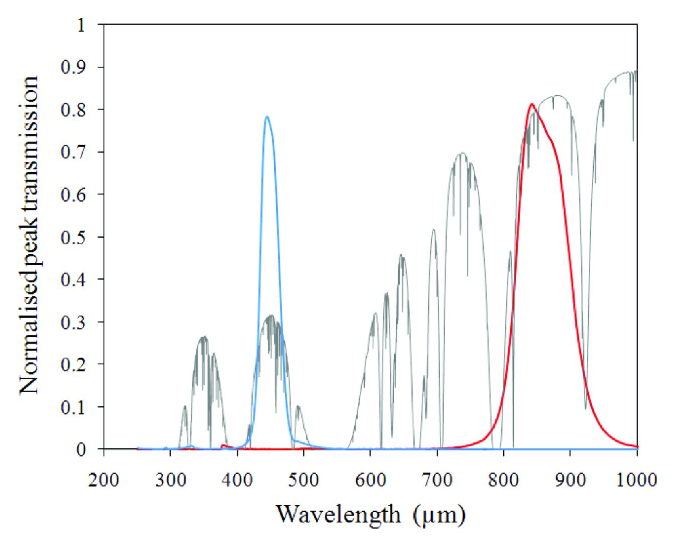
\includegraphics[width=\columnwidth]{ch1/Holland2013_transmission_plot.eps}
  \caption[Atmospheric transmission as a function of frequency at the summit of Mauna Kea]{A plot of the fraction of submillimetre emission that passes through the atmosphere as a function of wavelength at the summit of Mauna Kea, Hawaii (altitude approximately 4000~m).  The blue and red curves show the filter profiles of the 450 and 850~$\mu$m bands, respectively, of the SCUBA-2 instrument mounted on the JCMT.  \emph{Image credit: Figure~3 from Holland, W.~S.~et al., 2013, "SCUBA-2: The 10000 pixel bolometer camera on the James Clerk Maxwell Telescope", Monthly Notices of the Royal Astronomical Society, Volume 430, Issue 4, Pages 2513-2533.  Reproduced with permission from the Monthly Notices of the Royal Astronomical Society and Oxford University Press.}
  \label{fig:atmos_trans}}
 \end{center}
\end{figure}

%%%%%%%%%%%%% ISM
\section{The Interstellar Medium} \label{ism}
The interstellar medium (ISM) of a galaxy is a complex, multiphase environment, comprised primarily of gas and dust components and permeated by radiation at energies across much of the electromagnetic spectrum.  Its evolution with time is driven by the dynamics of the galaxy, and more importantly for the purposes of this thesis, star formation and subsequent feedback \citep{2005pcim.book.....T}.  Young star clusters rich in young, massive O and B stars provide a source of strong stellar winds and an outward flux of ionising radiation directed toward the surrounding gas and dust, impacting the physical characteristics of these components \citep{2007ARA&A..45..481Z}.  Furthermore, the violent death of these high-mass stars in supernova explosions deposits mechanical energy and material back into the ISM, which in turn recycles this matter into the next generation of stars.  We summarise the gas and dust components relevant to this thesis below.

\subsection{Interstellar Gas} \label{gas}
Interstellar gas permeates a galaxy and exists in a number of phases with a broad range of temperatures, and densities, and can be in both neutral and ionised states.  The bulk of the mass of a star-forming galaxy comprises hydrogen, both atomic (H~\textsc{i}) and molecular (H$_{2}$), though the relative contributions of each varies from galaxy to galaxy \citep{1989ApJ...347L..55Y,2002A&A...384...33B, 2009MNRAS.394.1857O}.  A wealth of atomic and molecular species make up the remaining fraction of gas.  Here we briefly describe the major components of the ISM and the typical ways to observe them.

The coldest gas is located within molecular clouds, the sites of star formation.  The temperature in these regions is very cold, typically 10~K \citep{1991ARA&A..29..581Y}, and the typical gas density is of the order $10^{2}$~cm$^{-3}$ \citep{2012arXiv1210.6990S}, which allows for the formation of molecules.  Molecular hydrogen comprises the majority of the gas in these clouds, followed by carbon monoxide (CO), the second most common molecule \citep[e.g.][]{1982ApJ...262..590F}.  In the densest regions other common molecular constituents include HCN, CS, HCO$^{+}$ and NH$_{3}$ \citep{2005pcim.book.....T,2007ARA&A..45..339B,2012arXiv1210.6990S}.  Star formation occurs in embedded cores within these clouds, where the conditions are different than the rest of the cloud.

Immediately surrounding regions of star formation are low density, ionised environments called H~\textsc{ii} regions.  The harsh radiation field emanating from the central stars gives rise to hot gas temperatures of approximately $10^{4}$~K \citep{1985ApJS...57..349R, 2005pcim.book.....T} and densities spanning from tens to 10$^{4}$ particles~cm$^{-3}$ \citep{2005pcim.book.....T}.  A large fraction of photons from these hot, young stars are emitted in the ultraviolet waveband, and a smaller fraction emit in the X-ray regime, giving rise to the production of numerous ions with ionisation potentials greater than that of hydrogen (13.6~eV) including N$^{+}$, O$^{++}$, and H$^{+}$ \citep{2005pcim.book.....T}.

At increasingly larger distances from the star forming region, the radiation field is not as strong and the H~\textsc{ii} region transitions to a photon-dominated region (PDR).  Originally, a PDR was coined a photodissociation region by \citet{1985ApJ...291..722T} and was classically described to be the region adjacent to an H~\textsc{ii} region.  However, PDRs can encompass a wider range of environments and thus now a PDR is considered to be any region where far-ultraviolet photons (wavelength $\lambda = $912~\AA -- 2000~\AA ~or energy $E = $6--13.6~eV) dominate the chemistry in the gas \citep{1985ApJ...291..722T, 1991ApJ...377..192H}.  In fact, with this definition much of a galaxy's ISM exists in PDRs, and thus they are an important regime to study and understand in order to characterise the conditions within the ISM \citep{1985ApJ...291..722T}.

Temperatures within a PDR range from less than 100~K to upwards of a few thousand K \citep{1985ApJ...291..722T}, while densities can range from 10$^{1}$~cm$^{-3}$ to 10$^{6}$~cm$^{-3}$.  This diverse range of physical conditions in the gas within a PDR can be diagnosed by the presence of various atoms and ions.  Figure~\ref{fig:cloud} shows a cartoon representation of a molecular cloud with an embedded H~\textsc{ii} region and surrounding PDR.  In reality, the various environments are not so simply segregated, but this provides a basic description of conditions inside a molecular cloud.  


\begin{figure}[!h]
 \begin{center}
 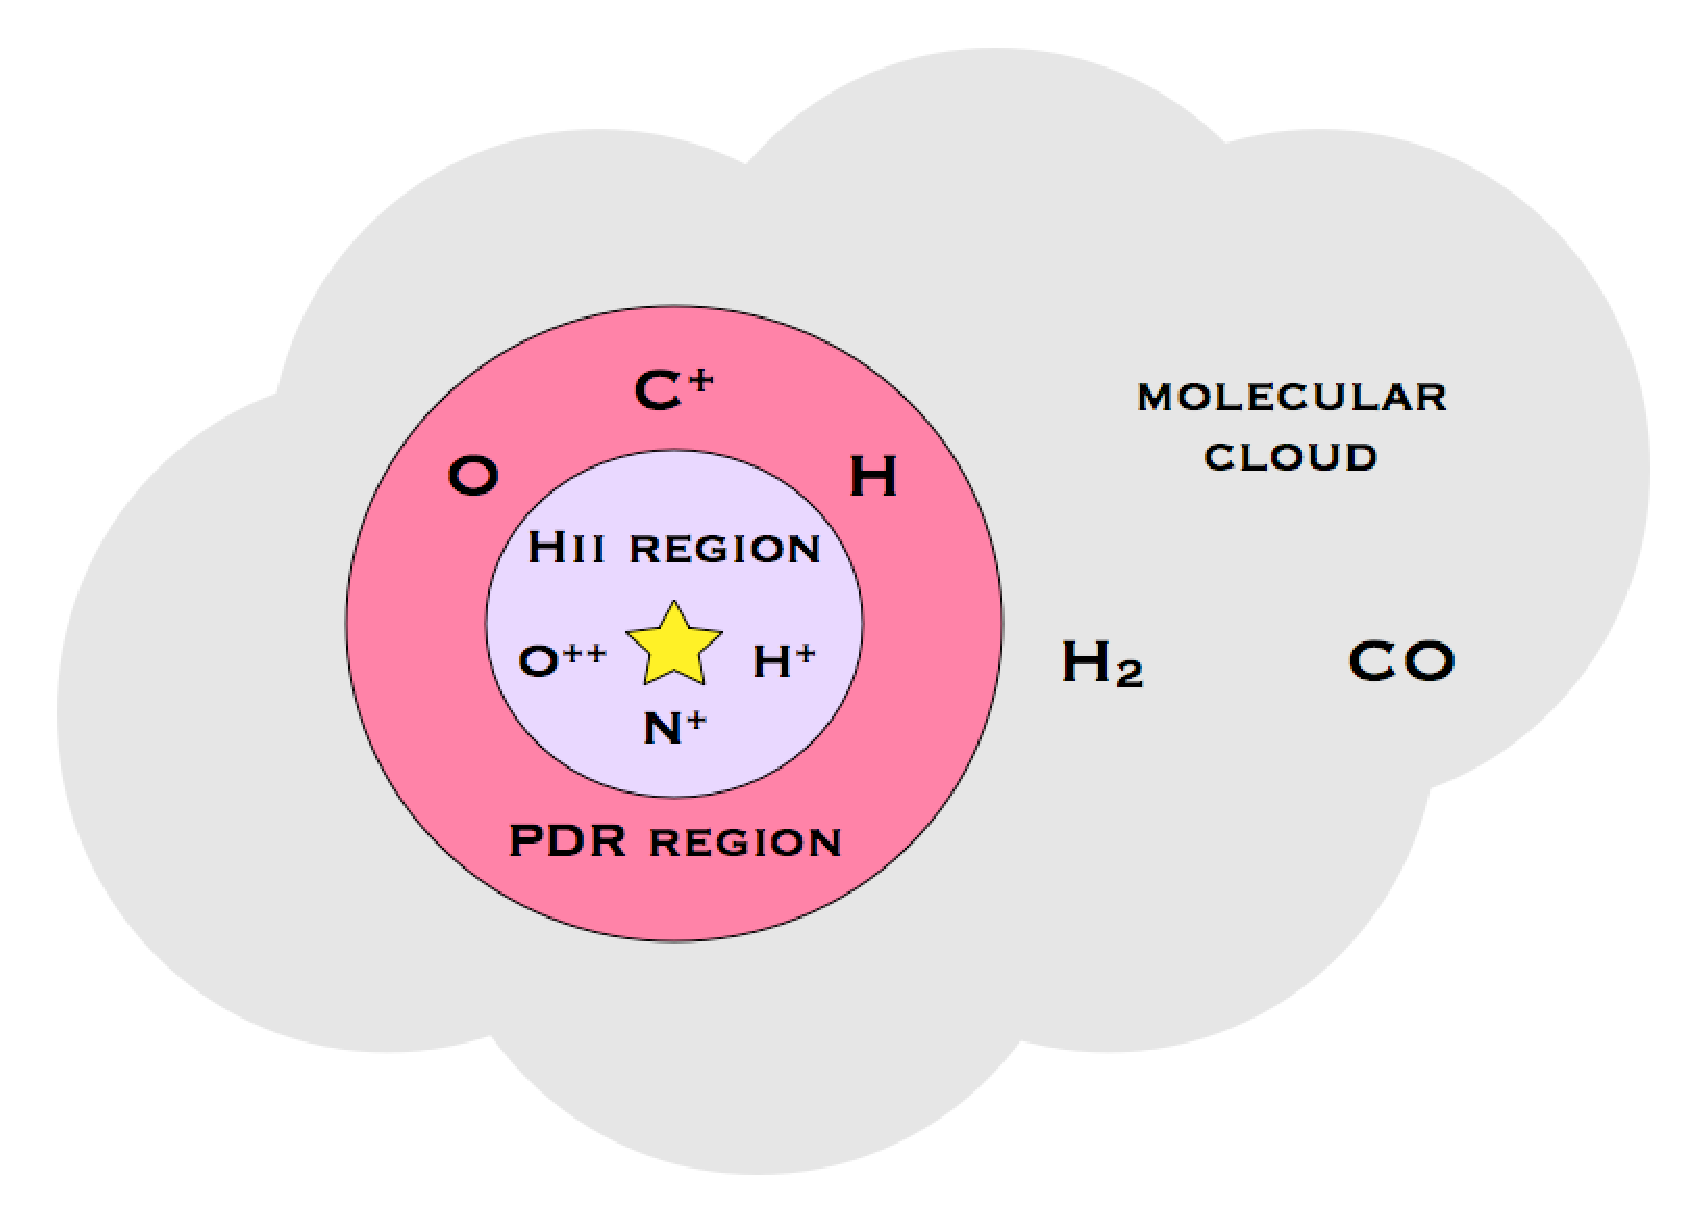
\includegraphics[width=\columnwidth]{ch1/molecular_cloud_schematic.eps}
  \caption[A cartoon of a molecular cloud]{A cartoon schematic of a molecular with an embedded stellar cluster and surrounding H~\textsc{ii} and PDR regions.
  \label{fig:cloud}}
 \end{center}
\end{figure}

\subsection{Important Gas Tracers} \label{gas_tracer}
Determining the physical conditions of the gas within the ISM involves observations of various atoms, ions and molecules and subsequent comparison of these observations with a theoretical model representing the ISM phase of interest.  Here we describe some of the most important gas tracers, how they are produced and how we observe them.

\subsubsection{Cold Gas}\label{cold_gas}
As stated above, the majority of a star forming galaxy's mass is found in neutral atomic and molecular hydrogen.  Atomic hydrogen is probed via the ``21~cm'' line using radio telescopes, and some of the earliest reports of observations of this line in our Milky Way are summarised by \citet{1951AJ.....56..144V}.  Studies of the H~\textsc{i} 21~cm line emission show that the atomic hydrogen distribution in galaxies is more extended than the optical disk \citep[e.g.][]{1997A&A...324..877B,2010ASPC..438....3T}.  The ubiquity of the atomic gas lends support to the importance of atomic hydrogen in understanding the properties of the ISM and the dynamics of a galaxy.  A morphological exception is early type galaxies (ellipticals and lenticulars), which often show few detections in atomic gas \citep[e.g.][]{1985AJ.....90..454K,1987IAUS..127..145K,1995A&A...300..675H,2010MNRAS.409..500O}.

Molecular gas is a more direct tracer of star formation than atomic gas, as star formation occurs in molecular clouds.  Observing molecular hydrogen (H$_{2}$) in its ground state is very difficult because it does not have an electric dipole moment \citep{1991ARA&A..29..581Y}.  Thus, we trace it indirectly using observations of the $J=1-0$ rotational transition of carbon monoxide (CO) and an empirically determined relation between the column density of H$_{2}$ and the integrated intensity of CO, the ``CO-to-H$_{2}$ conversion factor'', $X_{\mathrm{CO}}$ \citep[e.g.][]{1991ARA&A..29..581Y}.  The typical value of this conversion factor is $2 \times 10^{20}$~cm$^{-2}$~(K~km~s$^{-1}$)$^{-1}$ \citep{1988A&A...207....1S}, although this value is different in ultra luminous infrared galaxies \citep{1998ApJ...507..615D}, and can vary with radius and metallicity \citep[e.g. ][ and references therein]{2013arXiv1301.3498B}.  Higher level rotational transitions are useful tracers of warmer molecular gas \citep{2009ApJ...693.1736W}.  One way to observe molecular hydrogen directly is through its quadrupole moment rotational transitions, which produce spectral lines in the infrared \citep{1991ARA&A..29..581Y}, accessible through observatories such as \emph{Spitzer}.  It is also possible to observe H$_{2}$ directly via vibrational transitions of an electronically excited molecule, giving rise to spectral lines at around 2~$\mu$m \citep{2005pcim.book.....T}.  Lastly, one can observe H$_{2}$ absorption lines in the ultraviolet Lyman-Werner bands, which indicate upward electronic transitions \citep{2005pcim.book.....T}.

\subsubsection{H~\textsc{ii} regions and PDRs}\label{fine_lines}
Atomic fine structure lines are the most important spectral lines for tracing hot ionised gas in H~\textsc{ii} regions and the cool neutral gas in PDRs.  These lines contribute to the total cooling of the gas in their respective environments by removing thermal energy from the gas.  Gas heating occurs when radiation (usually FUV) from nearby stars provides photons which eject electrons from dust grains or polycyclic aromatic hydrocarbons (PAHs) via the photoelectric effect \citep{1985ApJ...291..722T,1991ApJ...377..192H}.  These free electrons subsequently contribute to the thermal energy of the gas.  Depending on the temperature of the gas, certain atoms and ions can be collisionally excited, and if the density of the gas is less than the critical density, which is the ratio of the spontaneous emission coefficient $A_{ij}$ divided by the collisional rate coefficient $\gamma_{ij}$, these excited atoms will most often emit a photon via a fine structure transition rather than collisionally de-excite, as shown in Figure~\ref{fig:cooling} \citep{2005pcim.book.....T}.

\begin{figure}[!h]
 \begin{center}
 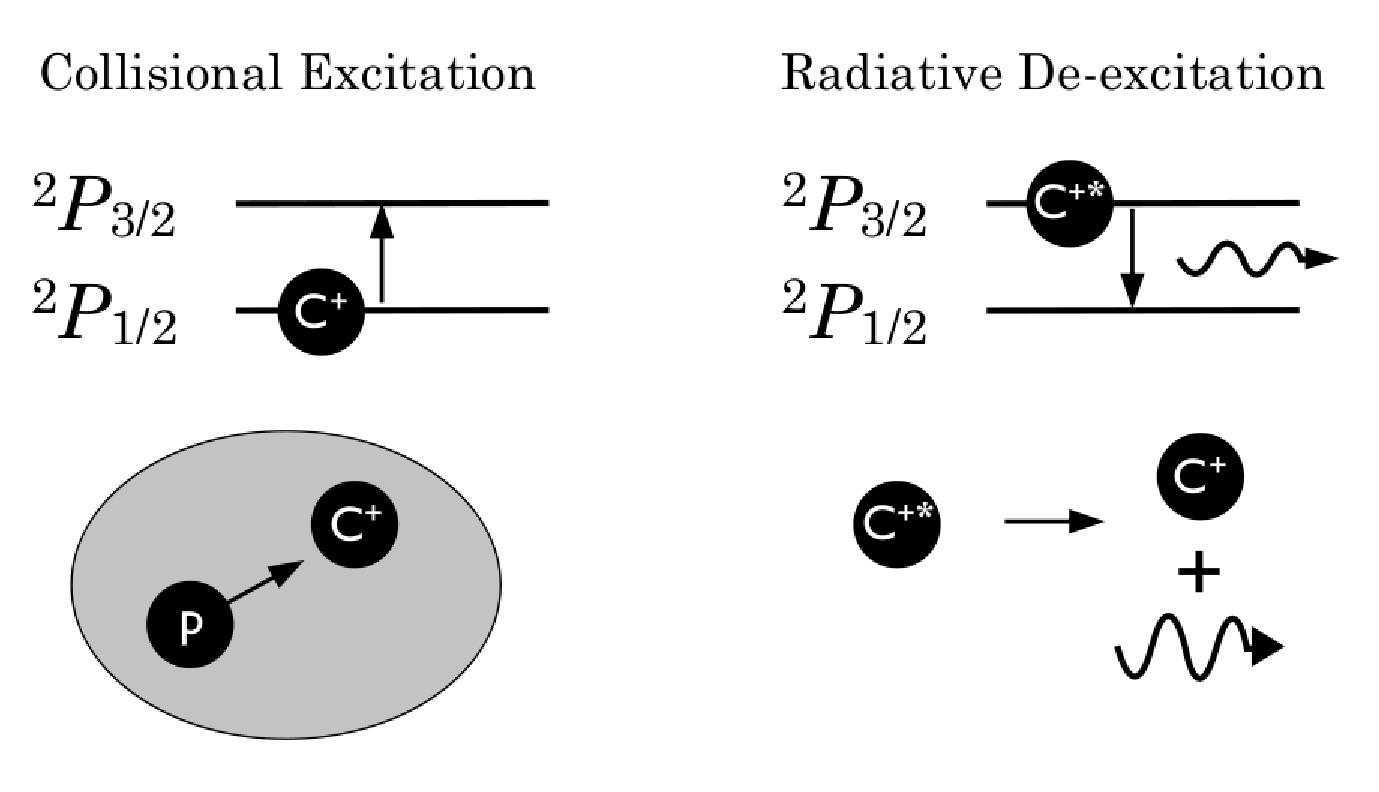
\includegraphics[width=\columnwidth]{ch1/cooling_line_schematic.eps}
  \caption[A cartoon of the cooling process via the \mbox{[C~\textsc{ii}](158~$\mu$m)} fine structure line]{A cartoon schematic of the collisional excitation and subsequent radiative de-excitation of a C$^{+}$ atom via the [C~\textsc{ii}](158~$\mu$m) transition.  The C$^{+}$ atom is collisionally excited by a collision with a particle such as a proton or electron and makes an upward transition from the $^{2}P_{1/2}$ state to the $^{2}P_{3/2}$ state.  The excited carbon ion, C$^{+*}$, then returns to the ground state by emitting a photon, thus removing thermal energy from the gas.
  \label{fig:cooling}}
 \end{center}
\end{figure}

In an H~\textsc{ii} region the radiation field is hard enough to ionise atoms or ions with ionisation potentials greater than 13.6~eV, such as N$^{+}$, N$^{++}$ and O$^{++}$.  Among the brightest mid- and far-infrared cooling lines in these regimes are the [N~\textsc{ii}] lines at 122 and 205~$\mu$m, the [O~\textsc{iii}] line at 88~$\mu$m, and the [N~\textsc{iii}] line at 57~$\mu$m, although there are many more cooling lines that contribute to the overall energy balance of the ionized gas \citep[e.g. ][]{2001ApJ...553..121H,2012A&A...548A..20C,2012A&A...548A..91L}.

In the neutral gas within PDRs the excited atoms have ionisation potentials less than 13.6~eV.  Here, species such as C, C$^{+}$, O and CO are the important coolants. The [C~\textsc{ii}] fine structure line at 158~$\mu$m dominates the cooling in this environment in most normal galaxies, contributing roughly 1~\% of the total cooling budget of a galaxy \citep{1985ApJ...291..755C,1991ApJ...373..423S,2001ApJ...561..766M}; however, it can be suppressed in ultraluminous infrared galaxies \citep[e.g. ][]{1998ApJ...504L..11L,2003ApJ...594..758L}.  Other important PDR diagnostics include the [O~\textsc{i}] lines at 63 and 145~$\mu$m, and the various CO rotational transitions \citep{2001ApJ...561..766M,2001A&A...375..566N}.

\subsection{Interstellar Dust} \label{dust}
Dust is ubiquitous throughout the ISM and its thermal emission produces about half of the infrared continuum radiation observed in galaxies \citep{2010A&A...518L...1P}.  It is an important component of the ISM and molecular clouds in particular, as it shields strong radiation emitted by hot stars from penetrating deep into the cloud.  Dust also acts as a catalyst for the formation of H$_2$, polycyclic aromatic hydrocarbons (PAHs), and other molecules \citep{2005pcim.book.....T}.

The exact composition of dust grains is still debated in the literature but in general there is agreement that they fall into two broad categories, carbons and silicates (or other heavier non-carbon based grains), although a mixture of the two has also been put forth by some models.  Another important component, though not strictly dust grains but rather large molecules, is polycyclic aromatic hydrocarbons.  These are large planar molecules comprising carbon atom chains arranged in a hexagonal pattern with hydrogen atoms bonded to the outermost atoms, and their vibrational modes produce spectral lines at mid-infrared wavelengths \citep{1985ApJ...290L..25A}.

One of the pioneering dust models was put forth by \citet{1977ApJ...217..425M} to model the observed interstellar extinction curve, who proposed that the grain population comprised a mix of naked graphite particles plus particles of a different material such as silicates or iron-based particles.  They found that the observations were best matched by a model with a range in size of the dust grains between 0.005~$\mu$m to 1~$\mu$m for the graphites and 0.025 to 0.25~$\mu$m for the other grains, following a power law distribution.  Several later models have either adopted the size distribution of \citet{1977ApJ...217..425M} or further investigated the composition of the dust using only the graphite and silicate type dust grains \citep[e.g. ][]{1984ApJ...285...89D, 1994ApJ...422..164K}.  \citet{2001ApJ...554..778L} expanded the graphite and silicate model by adding a PAH component, represented by extending the grains down in size to as small as a few Angstroms in diameter and attributing to the very small carbonaceous grains the properties of PAHs.  One of the most recent models from this class is by \citet{2007ApJ...657..810D}, which is now commonly used by observers (see below).

Other dust modellers have attempted to fit observations with alternative types of dust grains.  For example, some authors such as \citet{1989ApJ...341..808M} consider `fluffy' dust grains that are a combination of amorphous carbon, graphite and silicate particles loosely stuck together, as well as particles comprising just graphite. Later, \citet{1996ApJ...472..643M} proposed a dust model of purely graphite, purely silicate, and fluffy composite grains of a mix of carbon, silicates and other elements. \citet{2004ApJS..152..211Z} consider a dust model with different sets of dust grain compositions (such as that of \citet{2001ApJ...554..778L}, one testing the effects of including amorphous carbon instead of graphite, one including other heavier composite grains, and even one with only PAHs and no large carbon-based grains) to reproduce several observational constraints, and find that multiple models adequately fit the observations, emphasising the difficulty in establishing the exact nature of the dust grains.  Lastly, a third model has been suggested that consists of dust grains with a silicate centre surrounded by a carbon-based coating, in addition to PAHs and carbon dominated very small grains \citep[e.g.][]{1990A&A...237..215D}.

As the dust grain modelling implies, grain sizes span a large range from small grains approximately 5~$\mbox{\AA}$ in diameter up to very large grains of approximately 1~$\mu$m.  Large grains are in thermodynamic equilibrium with their environment and emit radiation in the far-infrared and submillimetre wavebands, corresponding to temperatures of roughly 20~K \citep{2003ARA&A..41..241D}.  Smaller dust grains tend to be out of equilibrium with their surroundings and are stochastically heated due to their small size.  A single photon can significantly increase the temperature of a small dust grain, which then slowly re-radiates away that energy, thus producing a significant fraction of the radiation at wavelengths shorter than about 50~$\mu$m \citep{2003ARA&A..41..241D}.

Modelling the observed spectral energy distribution of a galaxy or region within a galaxy can reveal properties of the dust grains such as composition, temperature and approximate size, depending on the type of model one uses.  The simplest approach is to fit a modified blackbody (graybody) function, described by
\begin{equation}\label{eqn:bb}
 I(\nu,T) = C\nu^{\beta}B(\nu,T),
\end{equation}
to observed photometry at far-infrared to submillimetre wavelengths.  Here, $B(\nu,T)$ is the Planck function, $\nu^{\beta}$ is from the empirical equation for the dust opacity, $\kappa_{\nu} = \kappa_{0}(\nu/\nu_{0})^{\beta}$, with $\beta$ the dust emissivity, and $C$ is a scaling constant encompassing the distance to the source, the dust mass, and the factor $\kappa_{0}/\nu_{0}^{\beta}$ from the dust opacity function.  From a theoretical perspective, $\kappa$ and $\beta$ are functions of the properties of the dust grains \citep[e.g.][]{1984ApJ...285...89D} and thus $\kappa_0$ may be calculated using a dust grain model for $\nu_0$ \citep{2001ApJ...554..778L}.  The factor $\beta$ is often left as a free parameter when fitting observations, but a value of $\beta=2.0$ is a common result \citep[e.g. ][]{1995ApJ...451..188R,2003AJ....125.2361B,2012A&A...540A..54B,2012MNRAS.421.2917F}.  Thus, $\beta$ can also be fixed at 2.0 when modelling observations.

The other common way to model the dust SED of a galaxy is to incorporate a more sophisticated dust model into the fitting.  The most commonly used of these models is that of \citet{2007ApJ...657..810D}, which updates some of the properties of the dust grain models of \citet{2001ApJ...554..778L} and \citet{2001ApJ...548..296W}.  This model considers dust grains comprised of silicates, carbonaceous grains, and PAHs and parameterises the radiation field the dust is exposed to by a parameter $U$, which is a dimensionless quantity such that $u_{\nu} = Uu_{\nu}^{\mathrm{MW}}$ is the energy density of the field and $u_{\nu}^{\mathrm{MW}}$ is the energy density in the Solar neighbourhood from \citet{1983A&A...128..212M}.  The bulk of the interstellar dust (represented by a fraction $(1-\gamma)$) is exposed to a radiation field with a scaling factor of $U_{\mathrm{min}}$, while dust in the vicinity of PDRs (represented by a fraction $\gamma$) is exposed to an effective radiation field represented by a power-law distribution of radiation fields with scaling factors between $U_{\mathrm{min}}$ and $U_{\mathrm{max}}$.  Fitting the model to observed photometry can produce a best-fitting model spectrum and return information on several free parameters, namely $U_{\mathrm{min}}$, $\gamma$ and the fractional abundance of PAHs, $q_{\mathrm{PAH}}$, which in turn can be used to calculate secondary information such as the total dust mass.

Another dust SED model in the literature is that of \citet{1990A&A...237..215D}.  It too considers silicate, carbonaceous and PAH grains, although in this model the silicate grains are coated or mixed with carbonaceous material, rather than being purely silicate as is the case for the \citet{2007ApJ...657..810D}.  This model has three components that are allowed to vary to best fit the observed spectrum, namely the PAH spectrum, the very small grain (carbon dominated grains) spectrum, and the big grain (silicate-carbon composite) spectrum.  However, it requires that the radiation field be first calculated then entered as an input parameter, rather than being integrated into the code itself.  This work became the basis for the model of \citet{2001ApJ...549..215D}, who first introduced the parameterisation of the radiation field with $U$, and more recently that of \citet{2011A&A...536A..88G}, although that particular model was designed to work with low-metallicity environments.

%%%%%%%%%%%%% Galaxies
%Furthermore, they are often found in groups \citep{1983ApJS...52...61G}, such as our own Local Group, and clusters of galaxies such as the Virgo Cluster.
\section{The Interstellar Medium of Galaxies}\label{galaxies}
Galaxies come in a wide variety of morphological shapes and sizes, presenting us with a wealth of environments to study.  Based on their optical appearances they are classified loosely as either spiral galaxies, elliptical and lenticular galaxies, and in some cases, irregular galaxies \citep{1926ApJ....64..321H}.  Here we discuss briefly the basic properties of galaxies in each of the two major categories and give some details for the individual galaxies M51 and Centaurus~A, which are the particular focus of this thesis.

\subsection{Spiral Galaxies}\label{spirals}
Spiral or disk galaxies each consist of a disk, a central bulge, and a halo \citep{1998gaas.book.....B}, and vary in total mass between $10^{9}$ and $10^{12}$~M$_{\odot}$ \citep{carrol_ostlie}.  The disk is rich in gas (atomic and molecular) and dust and can extend as large as 50~kpc in radius \citep{carrol_ostlie}. The disk typically shows a spiral structure with arms extending outward from the centre or central bar; these arms appear more luminous at numerous wavelengths than the interarm regions due to an increase in ISM density and star formation.  These arms can vary in prominence from the grand-design style consisting of two distinct, symmetric arms, to flocculent, patchy arms \citep[e.g.][]{1926ApJ....64..321H,1982MNRAS.201.1021E,1987ApJ...314....3E,1998gaas.book.....B}.  The disk also contains a young stellar population in contrast to the bulge, which contains an older stellar population \citep[e.g.][]{1944ApJ...100..147B}.  The bulge is a spheroidal shape extending above and below the plane and can vary in size relative to the disk, often characterized by the bulge-to-disk ratio.   At the very centre of the bulge in most spiral galaxies are supermassive black holes, and some of these power active galactic nuclei, which expel energy outward via jets, radiation or wind \citep{2012ARA&A..50..455F}.  Lastly, the halo is a low density spheroidal region in which the disk sits.  It contains a population of globular clusters, old stars and dark matter \citep{1987AJ.....93..816K,1998gaas.book.....B}.  However, it is worthwhile noting that most galaxies are dark matter dominated everywhere, not just in the halo.

A number of surveys over the past decade have extensively studied the properties of the ISM in extragalactic sources.  In spiral galaxies there is a broad range of characteristics.  Atomic and molecular gas masses can range anywhere from $1 \times 10^{7}$--$1.4 \times 10^{10}$~M$_{\odot}$ and $7 \times 10^{6}$--$6 \times 10^{9}$~M$_{\odot}$, respectively, in nearby galaxies \citep[e.g.][]{2008AJ....136.2563W,2009AJ....137.4670L}.  There is also a wide range in temperatures for the dust populations.  \citet{2012MNRAS.425..763G} investigated two dust components, a warm one and a cold one, and found a range of cold dust temperatures between 19 and 25.2~K, and a range of warm dust temperatures between 56 and 63~K.  The total dust mass in spiral type galaxies ranges from 10$^{6.39}$--10$^{8.57}$ as found by the \emph{Spitzer} Infrared Nearby Galaxy Survey \citep{2007ApJ...663..866D}, while the dust-to-gas mass ratio is on average about 0.007 (corresponding to a gas-to-dust ratio of roughly 140).  More recently, \citet{2012MNRAS.425..763G} report dust masses in spirals between $\sim 5 \times 10^{6}$ and $1.4 \times 10^{8}$~M$_{\odot}$ via fitting the dust spectral energy distribution with a modified blackbody.  Thus, spiral galaxies encompass a vast set of characteristics for their ISM properties.

\subsubsection{M51}\label{m51_general}
M51 (NGC~5194), also known as the Whirlpool Galaxy is an excellent example of a grand design, spiral galaxy and is located roughly 9.9~Mpc away \citep{2009AstL...35..599T}.  Its optical disk is approximately $11.2\arcmin \times 6.9\arcmin$ (32.3~kpc~$\times$~19.9~kpc) in size at the 25$^{th}$ magnitude surface brightness level, $D_{25}$ \citep{2003PASP..115..928K}, while its disk as observed in H~\textsc{i} extends $\sim 12.4\arcmin \times 10.0\arcmin$ (35.7~kpc~$\times$~28.8~kpc) with a total mass of $2.54 \times 10^{9}$~M$_{\odot}$ \citep{2008AJ....136.2563W}.  The molecular hydrogen, H$_{2}$, has a total mass of $2 \times 10^{9}$~M$_{\odot}$ covering roughly $9\arcmin \times 6\arcmin$ and well traces the H~\textsc{i} emission.  However, the ratio of atomic-to-neutral gas varies from 0.1 in the centre to 20 at the edges \citep{2007A&A...461..143S} indicating that the centre of the galaxy is molecular gas dominated but transitions to atomic gas dominated with increasing radius \citep{2007A&A...461..143S}.  Studies of H$\alpha$ and Pa$\alpha$ emission show over 1000 H~\textsc{ii} regions and a star formation rate of roughly 4~M$_{\odot}$~yr$^{-1}$ \citep{2001AJ....122.3017S}.  The galaxy also has a weak Seyfert~2 nucleus \citep{1997ApJS..112..315H}.

The dust content in M51 has been studied extensively at infrared wavelengths.  \citet{2005ApJ...633..871C} first presented the \emph{Spitzer} photometry from the \emph{Spitzer} Infrared Nearby Galaxy Survey \citep[SINGS; ][]{2003PASP..115..928K} at 3.6, 4.5, 5.8, 8.0, 24, 70 and 160~$\mu$m.  They find that the spiral arms are well defined at infrared wavelengths, tracing PAH emission and warm dust.  Combining the infrared data with ultraviolet and optical maps they determine that the 24~$\mu$m emission can be used as a local tracer of the star formation rate in M51 and determine a star formation rate surface density of 0.015~M$_{\odot}$~yr$^{-1}$~kpc$^{-2}$.  \citet{2007ApJ...671..333K} complemented this study by also making use of the \emph{Spitzer} infrared data to study the star formation rate law.  They find a strong linear correlation in log-log space between the star formation rate surface density and the total hydrogen gas mass surface density, with a slope ranging from 1.37--1.56, consistent with that of the Kennicutt-Schmidt law \citep[which has a slope of $1.4 \pm 0.15$; ][]{1998ApJ...498..541K}.  More recently, \citet{2012ApJ...755..165M} utilized previously obtained infrared observations with \emph{Herschel} photometry at 70, 160, 250, 350 and 500~$\mu$m to carry out a detailed study of the dust via spectral energy distribution modelling.  They found dust temperatures varying between 20 and 25~K, and a total dust mass of $1.2 \times 10^{8}$~M$_{\odot}$.  The average gas-to-dust mass ratio is $94 \pm 17$, close to the average Galactic value of roughly 160 \citep{2004ApJS..152..211Z}.  In the same study, it was determined that the most recent starburst episode in M51 was less than 500~Myr ago.  Merger interactions between galaxies often trigger star formation, as demonstrated by numerical simulations \citep[e.g.][]{1996ApJ...464..641M}, and in M51, observations of the stellar population reveal that blue supergiants are found along the tidal tail between M51 and its companion \citep{2009AstL...35..599T}, supporting this theory.

\subsection{Elliptical Galaxies}\label{ellip}
Unlike spiral galaxies, elliptical galaxies generally do not have an obvious disk and instead are spheroidal in shape with a wide range of masses, between 10$^{7}$ and 10$^{13}$~M$_{\odot}$ and sizes from 0.1~kpc to over 100~kpc across \citep{carrol_ostlie}.  Elliptical galaxies contain large amounts of dark matter with mass-to-light ratios of upwards of 100~L$_{\odot}$~M$^{-1}_{\odot}$ \citep{carrol_ostlie} and may contain many globuler cluster systems.  They also follow a characteristic surface brightness profile that falls off as radius$^{1/4}$ in optical bands \citep{1948AnAp...11..247D}, and generally contain smaller amounts of cold gas and dust than spiral galaxies \citep[e.g.][]{2004A&A...416...41X, 2010ApJ...725..100W,2011MNRAS.414..940Y,2012ApJ...748..123S}.

Once thought to contain very little ISM, we now know that a significant fraction of early type galaxies do, in fact, contain gas and dust.  The ATLAS$^{3\mathrm{D}}$ survey \citep{2011MNRAS.414..940Y}, consisting of a sample of 260 early type galaxies with a median stellar mass of $3 \times 10^{10}$~M$_{\odot}$, found a 20\% detection rate in CO emission, implying the presence of molecular gas.  Of those galaxies with molecular mass, the amount ranges between 10$^{7}$ and 10$^{9.3}$~M$_{\odot}$.  The \emph{Herschel} Reference Survey \citep{2010PASP..122..261B} determined that dust was present in 50\% of their sample using the 250~$\mu$m waveband as an indicator \citep{2012ApJ...748..123S}.  Typical dust temperatures in early type galaxies range between 16 and 32~K, while dust masses are approximately $10^{4.5}$--10$^{7}$~M$_{\odot}$ \citep{1998ApJ...499..670B,2012ApJ...748..123S}.

\subsubsection{Centaurus~A}\label{cena_general}
Centaurus~A is a giant elliptical galaxy with a prominent dust lane running through the centre of the galaxy, located 3.8~Mpc away \citep{2010PASA...27..457H}.  It has a triaxial morphology implying no preferred axis of rotation and is approximately 20$\arcmin$ (22.1~kpc) in diameter as seen in optical wavebands \citep{1998A&ARv...8..237I}.  The galaxy is also rich in globular clusters, with over 400 confirmed \citep{2007AJ....134..494W,2010ApJ...708.1335W}.  It is believed that the galaxy underwent a merger with a small spiral galaxy at some point during its past, resulting in the warped disk and peculiar overall appearance \citep{1944ApJ...100..147B,1993ApJ...412..550Q}.

The disk is rich in both atomic and molecular gas \citep[e.g.][]{1990ApJ...363..451E,1990AJ.....99.1781V,1992ApJ...391..121Q,2010A&A...515A..67S} with a total H~\textsc{i} mass of $\sim 4 \times 10^{8}$~M$_{\odot}$, and total H$_{2}$ mass of $\sim 4 \times 10^{8}$~M$_{\odot}$ \citep{2010PASA...27..463M}.  There have been shells detected in the outskirts of the galaxy (as far as 15$\arcmin$ (16.6~kpc) from the centre) in H~\textsc{i}, which strengthen the merger model \citep{1994ApJ...423L.101S}.  Infrared studies using \emph{Spitzer} IRAC observations by \citet{2006ApJ...645.1092Q} reveal a ring that resembles a parallelogram  as seen in the 3.6, 4.5, 5.8 and 8.0~$\mu$m wavebands.  It is modelled as a set of concentric rings at various inclinations giving rise to the warped disk morphology.

Cen~A also has a set of very large radio lobes powered by an active galactic nucleus.  The total area covered by the radio emission is roughly $8^{\circ} \times 4^{\circ}$ (530.6~kpc $\times$ 265.3~kpc) \citep{1997A&AS..121...11C}, though the prominent bubble shaped lobes extend roughly 5~kpc outward from the nucleus \citep{1998A&ARv...8..237I}.  The compact jets near the nucleus extend only about 1~pc from the centre \citep{1998A&ARv...8..237I}.  There is also a large amount of X-ray emission from Cen~A, spatially coincident with the nucleus, jets and lobes \citep[e.g.][]{1997ApJ...475..118T,2009ApJ...698.2036K}.

%%%%%%%%%%%%%% Herschel
\section{The Herschel Space Observatory} \label{herschel}
The first space observatory designed to observe the sky at mid- and far-infrared wavelengths was the \emph{Infrared Astronomical Satellite} (IRAS), which carried out an all-sky survey in 1983 at four wavelengths, 12, 25, 60 and 100~$\mu$m \citep{1984ApJ...278L...1N}.  This survey produced a number of catalogs containing upwards of $2.7 \times 10^{5}$ point sources and extended sources, as well as hundreds of spectra of select objects \citep{IRAS_supp}. Following the success of IRAS, the \emph{Infrared Space Observatory} (ISO), capable of both photometric and spectroscopic observations between 2.5 and 240~$\mu$m, was launched in 1995 \citep{1996A&A...315L..27K}.  ISO had numerous advantages over IRAS, including the ability for the observing community to propose for time on the telescope for their own projects.  During the same era as IRAS and ISO the \emph{Kuiper Airborne Observatory}, which started flying in 1975 \citep[e.g.][and references therein]{1979PASP...91..143H}, complemented the space-based observations by conducting regular flights observing the sky at high altitudes using a variety of instruments over its roughly 20 year lifetime.

Striving to produce increasingly higher resolution images of everything from embedded young stellar objects to high-redshift sources, the National Aeronautics and Space Administration (NASA) created the \emph{Spitzer Space Telescope} \citep[hereafter \emph{Spitzer}; ][]{2004ApJS..154....1W}, launched in 2003.  \emph{Spitzer} has a primary mirror with a diameter of 85~cm \citep{2004ApJS..154....1W}, and two photometers and a spectrometer on board.  The Infrared Array Camera (IRAC) conducted photometry at 3.6, 4.5, 5.8 and 8~$\mu$m \citep{2004ApJS..154...10F} and is still observing today at the two shortest wavelengths.  The Multiband Imaging Photometer for \emph{Spitzer} (MIPS) also conducted photometry, but at the mid- to far-infrared wavelengths 24, 70 and 160~$\mu$m \citep{2004ApJS..154...25R}, spanning the peak dust continuum emission.  Lastly, the Infrared Spectrograph (IRS) could obtain spectra between 5.3 and 38~$\mu$m \citep{2004ApJS..154...18H}.  \emph{Spitzer} ran out of the cryogen that kept the telescope at just a few degrees above absolute zero in 2009 \citep{2010SPIE.7731E..17C}, thus beginning the warm mission.  The end of \emph{Spitzer}'s cold mission paved the way for the next set of far-infrared observatories. In May of 2009, the \emph{Herschel Space Observatory} \citep[hereafter \emph{Herschel}; ][]{2010A&A...518L...1P} was launched by the European Space Agency (ESA) with some involvement by NASA, while the joint NASA and German Aerospace Center (DLR) flying \emph{Stratospheric Observatory for Infrared Astronomy} (SOFIA) was also inaugurated in 2010 \citep{2012ApJ...749L..17Y}.  The majority of data acquired for this thesis come from \emph{Herschel}, thus taking advantage of the best far-infrared data currently available for analysis.

The \emph{Herschel Space Observatory} has revolutionised our view of the Universe in the regime of the far-infrared and submillimetre astronomy.  The primary mirror is currently the largest in space at 3.5~m in diameter \citep{2010A&A...518L...1P}, and the observatory has three instruments capable of photometric and spectroscopic observations on board: the Photodetector Array Camera and Spectrometer \citep[PACS; ][]{2010A&A...518L...2P}, the Spectral and Photometric Imaging REceiver \citep[SPIRE; ][]{2010A&A...518L...3G}, and the Heterodyne Instrument for the Far Infrared \citep[HIFI; ][]{2010A&A...518L...6D}.  A summary of the major properties of each instrument in comparison to previous observatories is presented in Table~\ref{tbl:herschel_prop}.  PACS covers similar wavelength ranges to both \emph{Spitzer} and ISO, but at much higher angular resolution (see Table~\ref{tbl:herschel_prop}).  SPIRE's wavelength range covers longer wavelengths than have been observed before by a space observatory, and in some cases, for the first time ever.  Furthermore, the SPIRE Fourier Transform Spectrometer (FTS) has the major advantage of being able to obtain the complete spectrum of a target, rather than discrete parts of the spectrum centred on select spectral lines or wavelength ranges.  In contrast to both the PACS spectrometer and the SPIRE FTS, HIFI makes use of heterodyne receivers to collect continous spectra between 157 and 213~$\mu$m, and 240 and 625~$\mu$m using seven bands.  A selection of some of the most interesting scientific discoveries \emph{Herschel} has made, focusing on those most relevant to this thesis, are discussed below.

\begin{landscape}
\begin{deluxetable}{lccccc}
\tabletypesize{\small}
\tablecolumns{5}
\tablecaption{A comparison of \emph{Herschel} to previous space observatories \label{tbl:herschel_prop}}
\tablewidth{0pt}
\tablehead{
\colhead{Property} & \multicolumn{4}{c}{Observatory} \\
\colhead{} & \colhead{\emph{Herschel}\tablenotemark{a}} & \colhead{\emph{Spitzer}\tablenotemark{b}} & \colhead{ISO\tablenotemark{c}} & \colhead{IRAS\tablenotemark{d}} 
}
 \startdata
 Primary Mirror diameter (m) & 3.5 & 0.85 & 0.6 & 0.6 \\
 Photometric Wavebands   & 70, 100, 160 (PACS) & 3.6, 4.5, 5.8, 8 (IRAC) & 2.5--5.5, 4--18 (ISOCAM) & 12, 25, 60, 100 \\
 ($\mu$m)                & 250, 350, 500 (SPIRE) & 24, 70, 160 (MIPS) & 3--120, 50--240 (ISOPHOT) &  \\
 Spectroscopic Wavelength & 55--210 (PACS)   &  5.3--38 (IRS) & 2.4--45.2 (SWS) & 8--13, 11--23 \\
 ($\mu$m)                 & 157--625 (HIFI)  &                & 43--197 (LWS) &  \\
                          & 194--671 (SPIRE) &  &  &  \\
 Photometric FWHM ($\arcsec$) & & & \\
  of select wavelengths: & & & \\
 \quad $\sim$24--25~$\mu$m    &        --       & 6  & 23 & 240--360 \\
 \quad 60 or 70~$\mu$m   &   $5.5 \times 5.8$   & 18 & 50--60 & 240--360 \\
 \quad 100~$\mu$m        &   $6.7 \times 6.9$   & -- & $\sim 80$ & 240-360 \\
 \quad 160~$\mu$m\phm{ISOCAMgapgap} &   \phm{gap}$10.5 \times 12.0$\phm{gap} & \phm{gapgapgap}40\phm{gapgapgap} & \phm{gapgapgap}134\phm{gapgapgap} & \phm{gapgap}--\phm{gapgap}\\
 \enddata
 \tablenotetext{a}{PACS: \citet{2010A&A...518L...2P}, SPIRE: \citet{2010A&A...518L...2P}, HIFI: \citet{2010A&A...518L...6D}; PACS FWHM from the \citet{pacs_om}, SPIRE FWHM from the \citet{spire_om}}
 \tablenotetext{b}{IRAC: \citet{2004ApJS..154...10F}, MIPS: \citet{2004ApJS..154...25R}, IRS: \citet{2004ApJS..154...18H}}
 \tablenotetext{c}{ISOCAM: \citet{1996A&A...315L..32C}, SWS: \citet{1996A&A...315L..49D}, LWS: \citet{1996A&A...315L..38C}; FWHM values from The ISO Handbook \citep{ISO_handbook}.}
 \tablenotetext{d}{IRAS Explanatory Supplement \citep{IRAS_supp}}
\end{deluxetable}
\end{landscape}


\subsection{Herschel Science Highlights} \label{herschel_sci}
There were many goals across various categories within astronomy set for \emph{Herschel} before it was launched, and it has certainly met and arguably exceeded a number of them already.  The mission has just come to an end, but many more results are still to come as the data become fully exploited by the astronomy community.  Advances and discoveries have been made in a number of areas from young embedded stellar objects to the distant Universe.  For example, \citet{2012A&A...540A.125A} presented \emph{Herschel} observations of a debris disk around the star Fomalhaut that indicate that the star's disk is active in producing fluffy dust grains via collisions, giving us insight into the dynamics of exoplanetary systems.  On slightly larger scales, \emph{Herschel} observations are revealing more clues about star formation.  Initial analysis of two subregions of the Herschel Infrared GALactic plane survey \citep[Hi-Gal; ][]{2010PASP..122..314M, 2010A&A...518L.100M} by \citet{2010A&A...518L..97E} found a total of almost 1000 embedded cores, and SED modelling of a subset of these objects indicates a large fraction of them are forming high-mass stars despite possessing lower than critical core gas mass surface densities.  This critical threshold is a theoretical value for the surface density of the gas that cores must surpass in order to form massive stars, and is derived to be 1~g~cm$^{-2}$ \citep{2008Natur.451.1082K}.  \emph{Herschel}'s high resolution photometry has also revealed that molecular clouds are filled with a cobweb-like structure of filaments, which possess a characteristic width of 0.1~pc that likely stems from the dissipation of turbulence \citep{2011A&A...529L...6A}.  These filamentary structures also appear to be the primary hosts of star-forming regions within a molecular cloud.

\emph{Herschel} has also produced some spectacular observations of many well-known galaxies.  The HERschel Inventory of The Agents of Galaxy Evolution \citep[HERITAGE; ][]{2010A&A...518L..71M} team is investigating the Small and Large Magellanic Clouds (SMC and LMC, respectively) in search of understanding the evolution of the ISM in a low-metallicity environment, one that might mimic primordial galaxies at high redshift.  \citet{2010A&A...518L..71M} presented early science results for the LMC and determined that the dust grains are likely composed of amorphous carbon and silicates rather than graphite and silicates.  One interesting result that stemmed from the \emph{Herschel} photometry of the LMC is the first far-infrared and submillimetre detection of Supernova~1987A.  An investigation of this emission showed that the dust coincident with the location of the remnant has been produced by the supernova ejecta, indicating quick processing of material post-event \citep{2011Sci...333.1258M}.  A study of the ultra-luminous infrared galaxy (ULIRG) Arp~220 by \citet{2011ApJ...743...94R} using the SPIRE Fourier Transform Spectrometer (FTS) revealed that this extreme environment hosts an X-ray luminous active galactic nucleus (AGN) at its centre and a wealth of molecules in various energy states in its gas component.  Furthermore, the mechanical energy of the merger in this galaxy is affecting this molecular gas.  The \emph{Herschel} Virgo Cluster Survey has presented numerous results thus far, one of which focuses on the dust-to-gas ratio of the spatially resolved members of the Virgo Cluster \citep{2012A&A...545A..75P}.  These authors find among other things a radially increasing or flat trend in the dust-to-gas ratio with increasing radius for galaxies deficient in atomic gas, and they conclude that the cluster environment is having an effect on the molecular gas and dust distributions within individual galaxy members.  The observations of the \emph{Herschel} Multi-tiered Extragalactic Survey have even revealed gravitationally lensed submillimetre galaxies, some of which would normally have fluxes too weak to be detected by SPIRE at 500~$\mu$m \citep{2013ApJ...762...59W}.

These are just a few of the many important and inspiring results published to date and there will be many more to come.  In this thesis, we focus on a unique set of observations from the PACS and SPIRE instruments, adding to the rich and diverse science produced with \emph{Herschel}.



%%%%%%%%%%%%%%%% PACS processing
\section{PACS Spectroscopy and Processing} \label{pac_spec}
A large portion of this thesis is spent analysing spectroscopy from the \emph{Herschel} PACS instrument; thus, it is useful to describe the data processing steps in more detail here than it appears in Chapters~\ref{chapter3} and \ref{chapter4}.  We refrain from detailing the PACS and SPIRE photometry reduction process further, as it is a more simple process and it is described sufficiently in Chapter~\ref{chapter2}.

The PACS spectrometer consists of 25 spatial pixels (spaxels) arranged in a $5 \times 5$ grid, with each spaxel covering a field of view on the sky of $9.4 \arcsec \times 9.4 \arcsec$ \citep{pacs_om}.  The spectral dimension in each spaxel is subdivided into 16 pixels, producing a spectral resolution of between approximately 75 and 300~km~s$^{-1}$ \citep{pacs_om}.  All of our PACS spectroscopic observations were carried out using the Line Spectroscopy mode, meaning we centred each observation on the spectral line we intended to target and the total wavelength range seen by the instrument was narrow, ranging from $\sim 0.35$--1.8~$\mu$m.  This wavelength range is stepped through by the instrument's grating during an observation such that each spaxel contains many individual spectra covering slightly different overlapping wavelength ranges, with the centre of the line being sampled by the most steps.  An example of these overlapping spectra for our [C~\textsc{ii}](158~$\mu$m) observations of the centre of M51 is shown in Figure~\ref{fig:data_cloud}.

\begin{figure}[!h]
 \begin{center}
 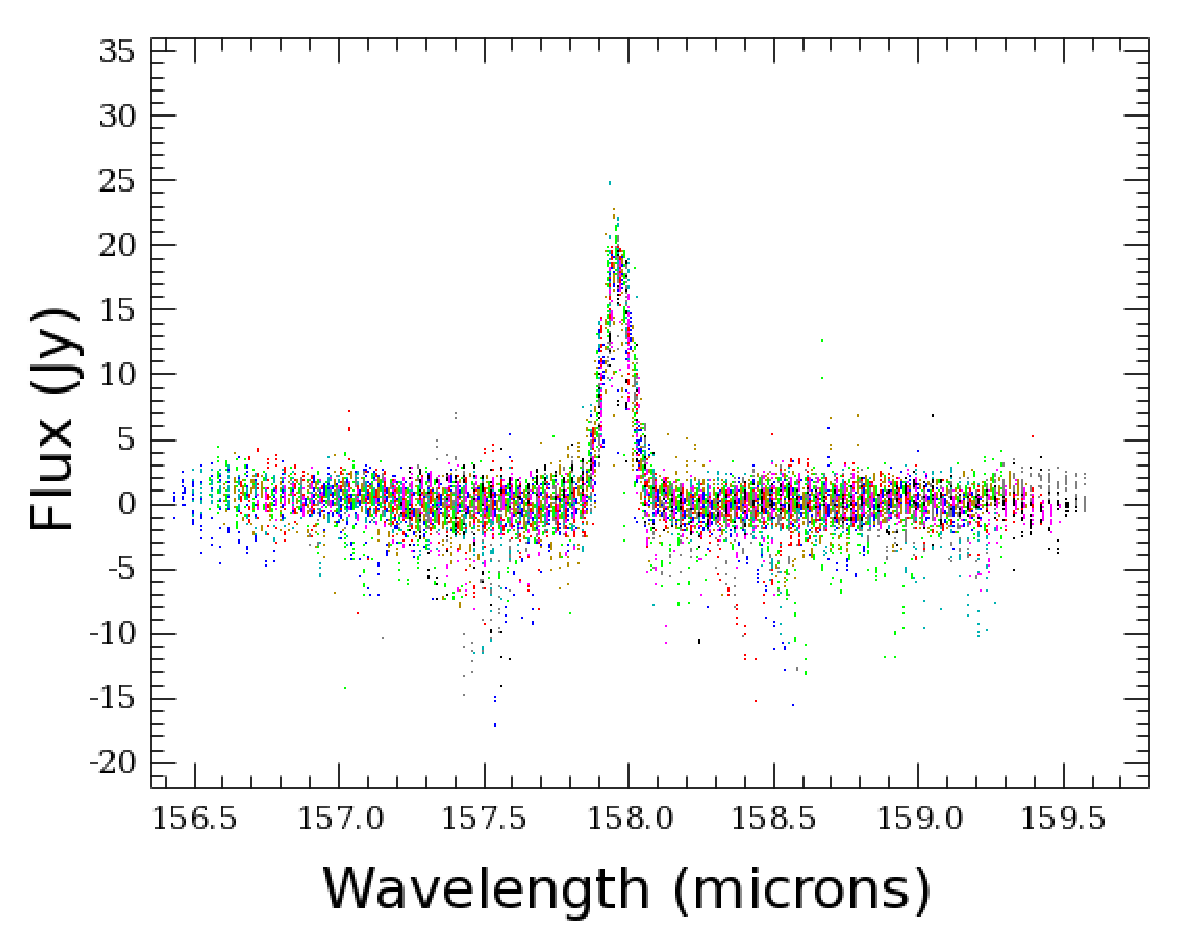
\includegraphics[width=\columnwidth]{ch1/M51_line_CII157.eps}
  \caption[Raw data cloud of a PACS \mbox{[C~\textsc{ii}](158~$\mu$m)} observation for M51]{An example of a PACS spectroscopic observation in its raw data form.  Shown is the spectrum of the [C~\textsc{ii}](158~$\mu$m) line in the central spaxel of one of the rasters of M51.
  \label{fig:data_cloud}}
 \end{center}
\end{figure}

The spectroscopic observations from the \emph{Herschel} PACS are initially processed using the Herschel Interactive Processing Environment \citep[HIPE; ][]{2010ASPC..434..139O} and Flexible Image Transport System (FITS) files holding the final spectral data are produced.  The line fitting and map making are done in a program called PACSman \citep{2012A&A...548A..91L}, which is an Interactive Data Language (IDL) package.

The line fitting iterates through each of the 25 spaxels comprising a single raster, and then through each raster if there is more than one, as is the case for both M51 (see Chapter~\ref{chapter3}) and Centaurus~A (see Chapter~\ref{chapter4}).  The fitting is carried out on the raw data produced in HIPE, prior to any rebinning, so as to obtain the best fit possible.  The continuum is fit first using a polynomial of up to a maximum of five orders, at the choice of the user.  For our observations, a second order polynomial was sufficient for the baseline fitting.  Next, the line is fit using a Gaussian function with the option of adding a broadening component for broader lines.  The parameters of the best fitting function, as well as the integrated flux, velocity information, full-width at half-maximum (FWHM) of the line, and continuum information are saved for the last step, map making.  An example of a [C~\textsc{ii}](158~$\mu$m) spectrum for M51 and its best fit are shown in Figure~\ref{fig:spectrum}.

\begin{figure}[!h]
 \begin{center}
 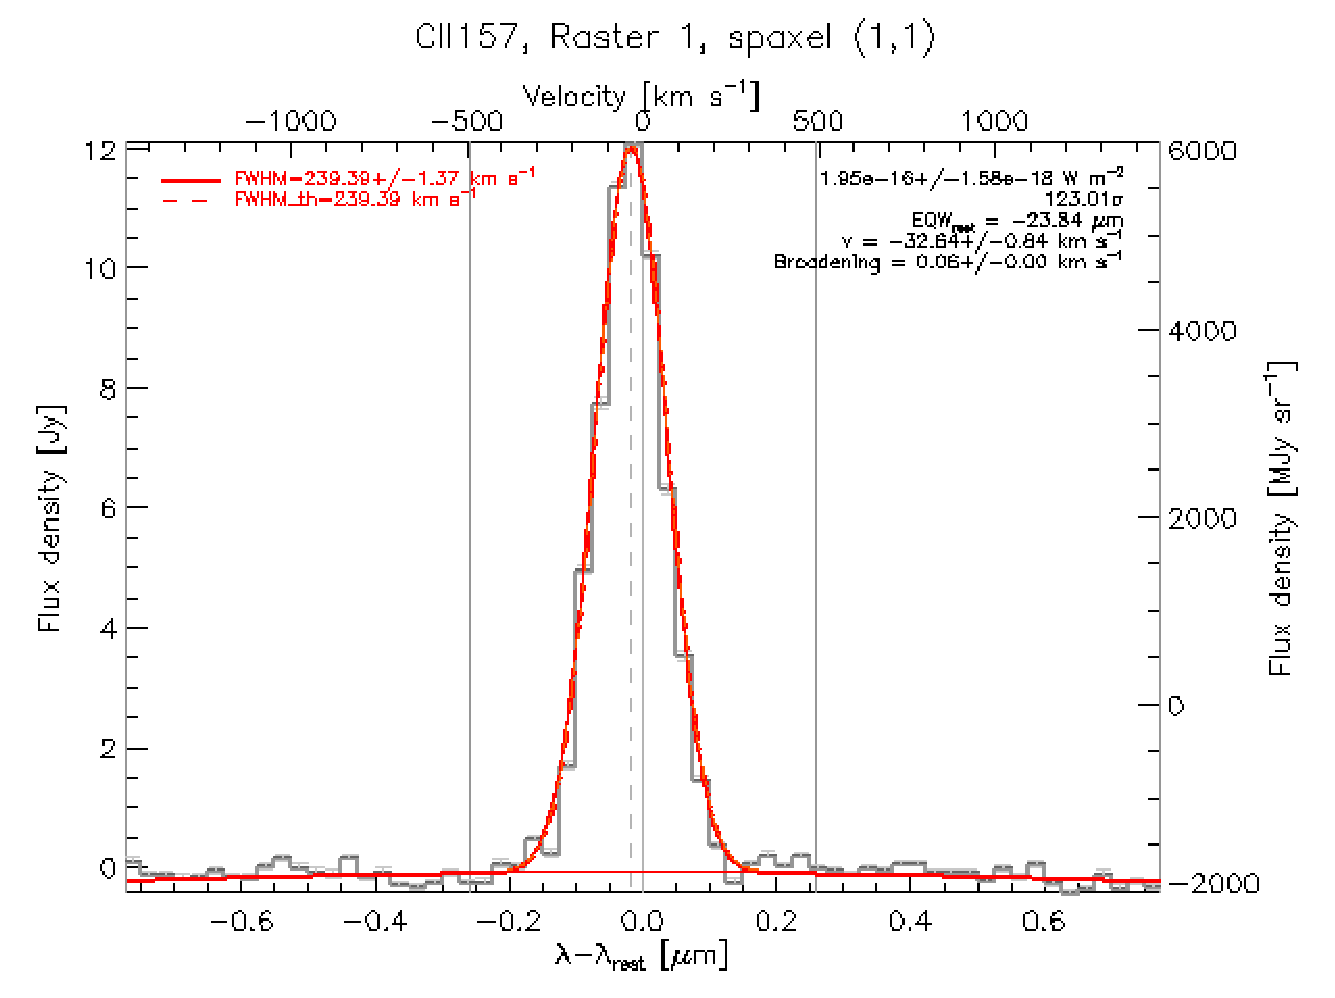
\includegraphics[width=\columnwidth]{ch1/M51_raster1_11.eps}
  \caption[Best line fit to a spaxel from PACS \mbox{[C~\textsc{ii}](158~$\mu$m)} observations of M51]{An example of a line fit to a [C~\textsc{ii}](158~$\mu$m) spectrum of M51 using PACSman.  The rebinned spectrum is shown in gray, the thin red line shows the best fit to the continuum, and the thick red line shows the best fit to the line.  The vertical gray lines mark the predicted line centre, and the two boundaries of the line component.  The vertical dashed line marks the observed line centre.
  \label{fig:spectrum}}
 \end{center}
\end{figure}

The maps are constructed by first laying down a grid with a pixel scale of $9.4 \arcsec /3$, corresponding to one-third of the original pixel scale of a raster (i.e. each pixel is subdivided into nine pixels at the new scale).  For each pixel in the final grid, the code iterates through all rasters searching for all contributing pixels.  Each contributing pixel is rotated through the appropriate position angle to align it to the final grid.  Next, the area of each original pixel that coincides with the selected final pixel is calculated as the weight for that pixel.  Finally, the weighted mean of the values of the contributing pixels is calculated and stored in the new pixel.  This process is completed for the flux, velocity, FWHM and continuum data and the new maps are stored as fits files for full analysis, along with their associated error maps.

%%%%%%%%%%%%%%%%%%% thesis outline
\section{This Thesis}\label{thesis_outline}
As described above, the infrared and submillimetre wavelength regime is important for probing the cold ISM.  With the unprecedented resolution of \emph{Herschel} we can now investigate the evolution of the cold regions of the ISM and the impact of star formation on not only molecular clouds in our own Milky Way, but in nearby galaxies as well.  Resolving details on scales of a few hundred parsecs in other galaxies gives us additional insight into the characteristics of the ISM and we can search for variations in these important properties within a single galaxy.  Extragalactic studies also allow us to look at each galaxy as a whole to broaden our undestanding, something that can be difficult to exploit in our own Galaxy, depending on the wavelength regime being used.  Thus, we can also compare and contrast ISM properties between galaxies of different morphologies to see how environment impacts the local ISM.

The \emph{Herschel} Very Nearby Galaxies Survey (VNGS; P.I. Christine Wilson) is a diverse sample of 13 galaxies located closer than roughly 80~Mpc away.  Centaurus~A (Cen~A; NGC~5128) and M51 (NGC~5194) are both sources that are a part of this survey.  M51 is classified as a grand-design, late-type spiral, SAbc \citep{1991trcb.book.....D}, and is oriented almost face-on to our line of sight.  Cen~A is classified as a peculiar S0 giant elliptical galaxy \citep{1991trcb.book.....D} and contains an embedded, edge-on disk.  Thus, at first glance they are quite different in morphology; however, both have active nuclei (CenA is a proper AGN and M51 is a low luminosity AGN) and have been affected by merger events.  Investigating the ISM in each galaxy affords us the ability to both search for regional variations as well as global morphological influence on the ISM.  In particular, we can compare and contrast the molecular cloud properties of the two galaxies and evaluate the possible influence of an active nucleus, a merger event, or spiral arms on the evolution and properties of the ISM.

In this thesis, we utilise observational data obtained from the James Clerk Maxwell Telescope and the \emph{Herschel} Space Observatory to investigate the gas and dust components of the ISM in Cen~A and M51.  Both observatories target wavelengths in the far-infrared and submillimetre regimes, key wavebands to study to enrich our understanding of the ISM.  Photometry from \emph{Herschel} allows us to model the observed spectral energy distribution (SED) on smaller scales, as well as at longer wavelengths than other space observatories.  \emph{Herschel}'s spectroscopic instruments have improved sensitivity and resolution over observatories such as ISO, allowing us to detect weaker far-infrared cooling lines that may have been previously undetected, in addition to better observations of the strongest lines.  Furthermore, the JCMT's HARP-B instrument allows us to probe the CO($J=3-2$) transition, adding additional information about the gas to our investigation.  Thus, we will study these two objects with the best data available to satisfy our scientific goals of contributing to the understanding of the evolution of the ISM.

This thesis is organised in the following manner.  In Chapter~\ref{chapter2} we present an investigation of the gas-to-dust ratio in Cen~A using \emph{Herschel} PACS and SPIRE photometry, as well as spectroscopy from the JCMT.  In Chapter~\ref{chapter3} we present an investigation of the molecular cloud properties of the inner region of M51 using photodissociation (photon dominated) region modelling of PACS spectroscopy, and in Chapter~\ref{chapter4} we carry out photodissociation region modelling on a radial strip of the disk of Cen~A.  We summarise the achievements of this work and discuss future directions in Chapter~\ref{chapter5}.

%\chapterbib
%\bibliography{thesis_bib}
%\bibliographystyle{apj}

\begin{thebibliography}{133}
\expandafter\ifx\csname natexlab\endcsname\relax\def\natexlab#1{#1}\fi

\bibitem[{{Acke} {et~al.}(2012){Acke}, {Min}, {Dominik}, {Vandenbussche},
  {Sibthorpe}, {Waelkens}, {Olofsson}, {Degroote}, {Smolders}, {Pantin},
  {Barlow}, {Blommaert}, {Brandeker}, {De Meester}, {Dent}, {Exter}, {Di
  Francesco}, {Fridlund}, {Gear}, {Glauser}, {Greaves}, {Harvey}, {Henning},
  {Hogerheijde}, {Holland}, {Huygen}, {Ivison}, {Jean}, {Liseau}, {Naylor},
  {Pilbratt}, {Polehampton}, {Regibo}, {Royer}, {Sicilia-Aguilar}, \&
  {Swinyard}}]{2012A&A...540A.125A}
{Acke}, B., {Min}, M., {Dominik}, C., {et~al.} 2012, \aap, 540, A125

\bibitem[{{Allamandola} {et~al.}(1985){Allamandola}, {Tielens}, \&
  {Barker}}]{1985ApJ...290L..25A}
{Allamandola}, L.~J., {Tielens}, A.~G.~G.~M., \& {Barker}, J.~R. 1985, \apjl,
  290, L25

\bibitem[{{Arzoumanian} {et~al.}(2011){Arzoumanian}, {Andr{\'e}}, {Didelon},
  {K{\"o}nyves}, {Schneider}, {Men'shchikov}, {Sousbie}, {Zavagno}, {Bontemps},
  {di Francesco}, {Griffin}, {Hennemann}, {Hill}, {Kirk}, {Martin}, {Minier},
  {Molinari}, {Motte}, {Peretto}, {Pezzuto}, {Spinoglio}, {Ward-Thompson},
  {White}, \& {Wilson}}]{2011A&A...529L...6A}
{Arzoumanian}, D., {Andr{\'e}}, P., {Didelon}, P., {et~al.} 2011, \aap, 529, L6

\bibitem[{{Baade}(1944)}]{1944ApJ...100..147B}
{Baade}, W. 1944, \apj, 100, 147

\bibitem[{{Bendo} {et~al.}(2003){Bendo}, {Joseph}, {Wells}, {Gallais}, {Haas},
  {Heras}, {Klaas}, {Laureijs}, {Leech}, {Lemke}, {Metcalfe}, {Rowan-Robinson},
  {Schulz}, \& {Telesco}}]{2003AJ....125.2361B}
{Bendo}, G.~J., {Joseph}, R.~D., {Wells}, M., {et~al.} 2003, \aj, 125, 2361

\bibitem[{{Bergin} \& {Tafalla}(2007)}]{2007ARA&A..45..339B}
{Bergin}, E.~A., \& {Tafalla}, M. 2007, \araa, 45, 339

\bibitem[{{Binney} \& {Merrifield}(1998)}]{1998gaas.book.....B}
{Binney}, J., \& {Merrifield}, M. 1998, {Galactic Astronomy}, Princeton Series
  in Astrophysics (Princeton, NJ: Princeton University Press)

\bibitem[{{Bolatto} {et~al.}(2013){Bolatto}, {Wolfire}, \&
  {Leroy}}]{2013arXiv1301.3498B}
{Bolatto}, A.~D., {Wolfire}, M., \& {Leroy}, A.~K. 2013, ArXiv e-prints

\bibitem[{{Boselli} {et~al.}(2002){Boselli}, {Lequeux}, \&
  {Gavazzi}}]{2002A&A...384...33B}
{Boselli}, A., {Lequeux}, J., \& {Gavazzi}, G. 2002, \aap, 384, 33

\bibitem[{{Boselli} {et~al.}(2010){Boselli}, {Eales}, {Cortese}, {Bendo},
  {Chanial}, {Buat}, {Davies}, {Auld}, {Rigby}, {Baes}, {Barlow}, {Bock},
  {Bradford}, {Castro-Rodriguez}, {Charlot}, {Clements}, {Cormier}, {Dwek},
  {Elbaz}, {Galametz}, {Galliano}, {Gear}, {Glenn}, {Gomez}, {Griffin}, {Hony},
  {Isaak}, {Levenson}, {Lu}, {Madden}, {O'Halloran}, {Okamura}, {Oliver},
  {Page}, {Panuzzo}, {Papageorgiou}, {Parkin}, {Perez-Fournon}, {Pohlen},
  {Rangwala}, {Roussel}, {Rykala}, {Sacchi}, {Sauvage}, {Schulz}, {Schirm},
  {Smith}, {Spinoglio}, {Stevens}, {Symeonidis}, {Vaccari}, {Vigroux},
  {Wilson}, {Wozniak}, {Wright}, \& {Zeilinger}}]{2010PASP..122..261B}
{Boselli}, A., {Eales}, S., {Cortese}, L., {et~al.} 2010, \pasp, 122, 261

\bibitem[{{Boselli} {et~al.}(2012){Boselli}, {Ciesla}, {Cortese}, {Buat},
  {Boquien}, {Bendo}, {Boissier}, {Eales}, {Gavazzi}, {Hughes}, {Pohlen},
  {Smith}, {Baes}, {Bianchi}, {Clements}, {Cooray}, {Davies}, {Gear}, {Madden},
  {Magrini}, {Panuzzo}, {Remy}, {Spinoglio}, \&
  {Zibetti}}]{2012A&A...540A..54B}
{Boselli}, A., {Ciesla}, L., {Cortese}, L., {et~al.} 2012, \aap, 540, A54

\bibitem[{{Bregman} {et~al.}(1998){Bregman}, {Snider}, {Grego}, \&
  {Cox}}]{1998ApJ...499..670B}
{Bregman}, J.~N., {Snider}, B.~A., {Grego}, L., \& {Cox}, C.~V. 1998, \apj,
  499, 670

\bibitem[{{Broeils} \& {Rhee}(1997)}]{1997A&A...324..877B}
{Broeils}, A.~H., \& {Rhee}, M.-H. 1997, \aap, 324, 877

\bibitem[{{Calzetti} {et~al.}(2005){Calzetti}, {Kennicutt}, {Bianchi},
  {Thilker}, {Dale}, {Engelbracht}, {Leitherer}, {Meyer}, {Sosey}, {Mutchler},
  {Regan}, {Thornley}, {Armus}, {Bendo}, {Boissier}, {Boselli}, {Draine},
  {Gordon}, {Helou}, {Hollenbach}, {Kewley}, {Madore}, {Martin}, {Murphy},
  {Rieke}, {Rieke}, {Roussel}, {Sheth}, {Smith}, {Walter}, {White}, {Yi},
  {Scoville}, {Polletta}, \& {Lindler}}]{2005ApJ...633..871C}
{Calzetti}, D., {Kennicutt}, Jr., R.~C., {Bianchi}, L., {et~al.} 2005, \apj,
  633, 871

\bibitem[{{Carey} {et~al.}(2010){Carey}, {Surace}, {Glaccum}, {Ingalls},
  {Krick}, {Lacy}, {Lowrance}, {Laine}, {O'Linger}, {Stauffer}, {Willner},
  {Hora}, {Hoffmann}, {Ashby}, {Huang}, {Marengo}, {Pahre}, {Wang}, {Werner},
  \& {Fazio}}]{2010SPIE.7731E..17C}
{Carey}, S.~J., {Surace}, J.~A., {Glaccum}, W.~J., {et~al.} 2010, in Society of
  Photo-Optical Instrumentation Engineers (SPIE) Conference Series, Vol. 7731,
  Society of Photo-Optical Instrumentation Engineers (SPIE) Conference Series

\bibitem[{{Carroll} \& {Ostlie}(2006)}]{carrol_ostlie}
{Carroll}, B.~W., \& {Ostlie}, D.~A. 2006, {An Introduction to Modern
  Astrophysics}, 2nd edn. (Addison-Wesley)

\bibitem[{{Cesarsky} {et~al.}(1996){Cesarsky}, {Abergel}, {Agnese}, {Altieri},
  {Augueres}, {Aussel}, {Biviano}, {Blommaert}, {Bonnal}, {Bortoletto},
  {Boulade}, {Boulanger}, {Cazes}, {Cesarsky}, {Chedin}, {Claret}, {Combes},
  {Cretolle}, {Davies}, {Desert}, {Elbaz}, {Engelmann}, {Epstein},
  {Franceschini}, {Gallais}, {Gastaud}, {Gorisse}, {Guest}, {Hawarden},
  {Imbault}, {Kleczewski}, {Lacombe}, {Landriu}, {Lapegue}, {Lena}, {Longair},
  {Mandolesi}, {Metcalfe}, {Mosquet}, {Nordh}, {Okumura}, {Ott}, {Perault},
  {Perrier}, {Persi}, {Puget}, {Purkins}, {Rio}, {Robert}, {Rouan}, {Roy},
  {Saint-Pe}, {Sam Lone}, {Sargent}, {Sauvage}, {Sibille}, {Siebenmorgen},
  {Sirou}, {Soufflot}, {Starck}, {Tiphene}, {Tran}, {Ventura}, {Vigroux},
  {Vivares}, \& {Wade}}]{1996A&A...315L..32C}
{Cesarsky}, C.~J., {Abergel}, A., {Agnese}, P., {et~al.} 1996, \aap, 315, L32

\bibitem[{{Clegg} {et~al.}(1996){Clegg}, {Ade}, {Armand}, {Baluteau}, {Barlow},
  {Buckley}, {Berges}, {Burgdorf}, {Caux}, {Ceccarelli}, {Cerulli}, {Church},
  {Cotin}, {Cox}, {Cruvellier}, {Culhane}, {Davis}, {di Giorgio}, {Diplock},
  {Drummond}, {Emery}, {Ewart}, {Fischer}, {Furniss}, {Glencross},
  {Greenhouse}, {Griffin}, {Gry}, {Harwood}, {Hazell}, {Joubert}, {King},
  {Lim}, {Liseau}, {Long}, {Lorenzetti}, {Molinari}, {Murray}, {Naylor},
  {Nisini}, {Norman}, {Omont}, {Orfei}, {Patrick}, {Pequignot}, {Pouliquen},
  {Price}, {Nguyen-Q-Rieu}, {Rogers}, {Robinson}, {Saisse}, {Saraceno},
  {Serra}, {Sidher}, {Smith}, {Smith}, {Spinoglio}, {Swinyard}, {Texier},
  {Towlson}, {Trams}, {Unger}, \& {White}}]{1996A&A...315L..38C}
{Clegg}, P.~E., {Ade}, P.~A.~R., {Armand}, C., {et~al.} 1996, \aap, 315, L38

\bibitem[{{Combi} \& {Romero}(1997)}]{1997A&AS..121...11C}
{Combi}, J.~A., \& {Romero}, G.~E. 1997, \aaps, 121, 11

\bibitem[{{Cormier} {et~al.}(2012){Cormier}, {Lebouteiller}, {Madden}, {Abel},
  {Hony}, {Galliano}, {Baes}, {Barlow}, {Cooray}, {De Looze}, {Galametz},
  {Karczewski}, {Parkin}, {R{\'e}my}, {Sauvage}, {Spinoglio}, {Wilson}, \&
  {Wu}}]{2012A&A...548A..20C}
{Cormier}, D., {Lebouteiller}, V., {Madden}, S.~C., {et~al.} 2012, \aap, 548,
  A20

\bibitem[{{Crawford} {et~al.}(1985){Crawford}, {Genzel}, {Townes}, \&
  {Watson}}]{1985ApJ...291..755C}
{Crawford}, M.~K., {Genzel}, R., {Townes}, C.~H., \& {Watson}, D.~M. 1985,
  \apj, 291, 755

\bibitem[{{Dale} {et~al.}(2001){Dale}, {Helou}, {Contursi}, {Silbermann}, \&
  {Kolhatkar}}]{2001ApJ...549..215D}
{Dale}, D.~A., {Helou}, G., {Contursi}, A., {Silbermann}, N.~A., \&
  {Kolhatkar}, S. 2001, \apj, 549, 215

\bibitem[{{de Graauw} {et~al.}(1996){de Graauw}, {Haser}, {Beintema},
  {Roelfsema}, {van Agthoven}, {Barl}, {Bauer}, {Bekenkamp}, {Boonstra},
  {Boxhoorn}, {Cote}, {de Groene}, {van Dijkhuizen}, {Drapatz}, {Evers},
  {Feuchtgruber}, {Frericks}, {Genzel}, {Haerendel}, {Heras}, {van der Hucht},
  {van der Hulst}, {Huygen}, {Jacobs}, {Jakob}, {Kamperman}, {Katterloher},
  {Kester}, {Kunze}, {Kussendrager}, {Lahuis}, {Lamers}, {Leech}, {van der
  Lei}, {van der Linden}, {Luinge}, {Lutz}, {Melzner}, {Morris}, {van Nguyen},
  {Ploeger}, {Price}, {Salama}, {Schaeidt}, {Sijm}, {Smoorenburg}, {Spakman},
  {Spoon}, {Steinmayer}, {Stoecker}, {Valentijn}, {Vandenbussche}, {Visser},
  {Waelkens}, {Waters}, {Wensink}, {Wesselius}, {Wiezorrek}, {Wieprecht},
  {Wijnbergen}, {Wildeman}, \& {Young}}]{1996A&A...315L..49D}
{de Graauw}, T., {Haser}, L.~N., {Beintema}, D.~A., {et~al.} 1996, \aap, 315,
  L49

\bibitem[{{de Graauw} {et~al.}(2010){de Graauw}, {Helmich}, {Phillips},
  {Stutzki}, {Caux}, {Whyborn}, {Dieleman}, {Roelfsema}, {Aarts}, {Assendorp},
  {Bachiller}, {Baechtold}, {Barcia}, {Beintema}, {Belitsky}, {Benz}, {Bieber},
  {Boogert}, {Borys}, {Bumble}, {Ca{\"\i}s}, {Caris}, {Cerulli-Irelli},
  {Chattopadhyay}, {Cherednichenko}, {Ciechanowicz}, {Coeur-Joly}, {Comito},
  {Cros}, {de Jonge}, {de Lange}, {Delforges}, {Delorme}, {den Boggende},
  {Desbat}, {Diez-Gonz{\'a}lez}, {di Giorgio}, {Dubbeldam}, {Edwards},
  {Eggens}, {Erickson}, {Evers}, {Fich}, {Finn}, {Franke}, {Gaier}, {Gal},
  {Gao}, {Gallego}, {Gauffre}, {Gill}, {Glenz}, {Golstein}, {Goulooze},
  {Gunsing}, {G{\"u}sten}, {Hartogh}, {Hatch}, {Higgins}, {Honingh}, {Huisman},
  {Jackson}, {Jacobs}, {Jacobs}, {Jarchow}, {Javadi}, {Jellema}, {Justen},
  {Karpov}, {Kasemann}, {Kawamura}, {Keizer}, {Kester}, {Klapwijk}, {Klein},
  {Kollberg}, {Kooi}, {Kooiman}, {Kopf}, {Krause}, {Krieg}, {Kramer},
  {Kruizenga}, {Kuhn}, {Laauwen}, {Lai}, {Larsson}, {Leduc}, {Leinz}, {Lin},
  {Liseau}, {Liu}, {Loose}, {L{\'o}pez-Fernandez}, {Lord}, {Luinge}, {Marston},
  {Mart{\'{\i}}n-Pintado}, {Maestrini}, {Maiwald}, {McCoey}, {Mehdi}, {Megej},
  {Melchior}, {Meinsma}, {Merkel}, {Michalska}, {Monstein}, {Moratschke},
  {Morris}, {Muller}, {Murphy}, {Naber}, {Natale}, {Nowosielski}, {Nuzzolo},
  {Olberg}, {Olbrich}, {Orfei}, {Orleanski}, {Ossenkopf}, {Peacock}, {Pearson},
  {Peron}, {Phillip-May}, {Piazzo}, {Planesas}, {Rataj}, {Ravera}, {Risacher},
  {Salez}, {Samoska}, {Saraceno}, {Schieder}, {Schlecht}, {Schl{\"o}der},
  {Schm{\"u}lling}, {Schultz}, {Schuster}, {Siebertz}, {Smit}, {Szczerba},
  {Shipman}, {Steinmetz}, {Stern}, {Stokroos}, {Teipen}, {Teyssier}, {Tils},
  {Trappe}, {van Baaren}, {van Leeuwen}, {van de Stadt}, {Visser}, {Wildeman},
  {Wafelbakker}, {Ward}, {Wesselius}, {Wild}, {Wulff}, {Wunsch}, {Tielens},
  {Zaal}, {Zirath}, {Zmuidzinas}, \& {Zwart}}]{2010A&A...518L...6D}
{de Graauw}, T., {Helmich}, F.~P., {Phillips}, T.~G., {et~al.} 2010, \aap, 518,
  L6

\bibitem[{{de Vaucouleurs}(1948)}]{1948AnAp...11..247D}
{de Vaucouleurs}, G. 1948, Annales d'Astrophysique, 11, 247

\bibitem[{{de Vaucouleurs} {et~al.}(1991){de Vaucouleurs}, {de Vaucouleurs},
  {Corwin}, {Buta}, {Paturel}, \& {Fouque}}]{1991trcb.book.....D}
{de Vaucouleurs}, G., {de Vaucouleurs}, A., {Corwin}, Jr., H.~G., {et~al.}
  1991, {Third Reference Catalogue of Bright Galaxies} (Springer-Verlag, New
  York)

\bibitem[{{Desert} {et~al.}(1990){Desert}, {Boulanger}, \&
  {Puget}}]{1990A&A...237..215D}
{Desert}, F.-X., {Boulanger}, F., \& {Puget}, J.~L. 1990, \aap, 237, 215

\bibitem[{{Downes} \& {Solomon}(1998)}]{1998ApJ...507..615D}
{Downes}, D., \& {Solomon}, P.~M. 1998, \apj, 507, 615

\bibitem[{{Draine}(2003)}]{2003ARA&A..41..241D}
{Draine}, B.~T. 2003, \araa, 41, 241

\bibitem[{{Draine} \& {Lee}(1984)}]{1984ApJ...285...89D}
{Draine}, B.~T., \& {Lee}, H.~M. 1984, \apj, 285, 89

\bibitem[{{Draine} \& {Li}(2007)}]{2007ApJ...657..810D}
{Draine}, B.~T., \& {Li}, A. 2007, \apj, 657, 810

\bibitem[{{Draine} {et~al.}(2007){Draine}, {Dale}, {Bendo}, {Gordon}, {Smith},
  {Armus}, {Engelbracht}, {Helou}, {Kennicutt}, {Li}, {Roussel}, {Walter},
  {Calzetti}, {Moustakas}, {Murphy}, {Rieke}, {Bot}, {Hollenbach}, {Sheth}, \&
  {Teplitz}}]{2007ApJ...663..866D}
{Draine}, B.~T., {Dale}, D.~A., {Bendo}, G., {et~al.} 2007, \apj, 663, 866

\bibitem[{{Eckart} {et~al.}(1990){Eckart}, {Cameron}, {Rothermel}, {Wild},
  {Zinnecker}, {Rydbeck}, {Olberg}, \& {Wiklind}}]{1990ApJ...363..451E}
{Eckart}, A., {Cameron}, M., {Rothermel}, H., {et~al.} 1990, \apj, 363, 451

\bibitem[{{Elia} {et~al.}(2010){Elia}, {Schisano}, {Molinari}, {Robitaille},
  {Angl{\'e}s-Alc{\'a}zar}, {Bally}, {Battersby}, {Benedettini}, {Billot},
  {Calzoletti}, {di Giorgio}, {Faustini}, {Li}, {Martin}, {Morgan}, {Motte},
  {Mottram}, {Natoli}, {Olmi}, {Paladini}, {Piacentini}, {Pestalozzi},
  {Pezzuto}, {Polychroni}, {Smith}, {Strafella}, {Stringfellow}, {Testi},
  {Thompson}, {Traficante}, \& {Veneziani}}]{2010A&A...518L..97E}
{Elia}, D., {Schisano}, E., {Molinari}, S., {et~al.} 2010, \aap, 518, L97

\bibitem[{{Elmegreen} \& {Elmegreen}(1982)}]{1982MNRAS.201.1021E}
{Elmegreen}, D.~M., \& {Elmegreen}, B.~G. 1982, \mnras, 201, 1021

\bibitem[{{Elmegreen} \& {Elmegreen}(1987)}]{1987ApJ...314....3E}
---. 1987, \apj, 314, 3

\bibitem[{{Fabian}(2012)}]{2012ARA&A..50..455F}
{Fabian}, A.~C. 2012, \araa, 50, 455

\bibitem[{{Fazio} {et~al.}(2004){Fazio}, {Hora}, {Allen}, {Ashby}, {Barmby},
  {Deutsch}, {Huang}, {Kleiner}, {Marengo}, {Megeath}, {Melnick}, {Pahre},
  {Patten}, {Polizotti}, {Smith}, {Taylor}, {Wang}, {Willner}, {Hoffmann},
  {Pipher}, {Forrest}, {McMurty}, {McCreight}, {McKelvey}, {McMurray}, {Koch},
  {Moseley}, {Arendt}, {Mentzell}, {Marx}, {Losch}, {Mayman}, {Eichhorn},
  {Krebs}, {Jhabvala}, {Gezari}, {Fixsen}, {Flores}, {Shakoorzadeh}, {Jungo},
  {Hakun}, {Workman}, {Karpati}, {Kichak}, {Whitley}, {Mann}, {Tollestrup},
  {Eisenhardt}, {Stern}, {Gorjian}, {Bhattacharya}, {Carey}, {Nelson},
  {Glaccum}, {Lacy}, {Lowrance}, {Laine}, {Reach}, {Stauffer}, {Surace},
  {Wilson}, {Wright}, {Hoffman}, {Domingo}, \& {Cohen}}]{2004ApJS..154...10F}
{Fazio}, G.~G., {Hora}, J.~L., {Allen}, L.~E., {et~al.} 2004, \apjs, 154, 10

\bibitem[{{Foyle} {et~al.}(2012){Foyle}, {Wilson}, {Mentuch}, {Bendo},
  {Dariush}, {Parkin}, {Pohlen}, {Sauvage}, {Smith}, {Roussel}, {Baes},
  {Boquien}, {Boselli}, {Clements}, {Cooray}, {Davies}, {Eales}, {Madden},
  {Page}, \& {Spinoglio}}]{2012MNRAS.421.2917F}
{Foyle}, K., {Wilson}, C.~D., {Mentuch}, E., {et~al.} 2012, \mnras, 421, 2917

\bibitem[{{Frerking} {et~al.}(1982){Frerking}, {Langer}, \&
  {Wilson}}]{1982ApJ...262..590F}
{Frerking}, M.~A., {Langer}, W.~D., \& {Wilson}, R.~W. 1982, \apj, 262, 590

\bibitem[{{Galametz} {et~al.}(2012){Galametz}, {Kennicutt}, {Albrecht},
  {Aniano}, {Armus}, {Bertoldi}, {Calzetti}, {Crocker}, {Croxall}, {Dale},
  {Donovan Meyer}, {Draine}, {Engelbracht}, {Hinz}, {Roussel}, {Skibba},
  {Tabatabaei}, {Walter}, {Weiss}, {Wilson}, \&
  {Wolfire}}]{2012MNRAS.425..763G}
{Galametz}, M., {Kennicutt}, R.~C., {Albrecht}, M., {et~al.} 2012, \mnras, 425,
  763

\bibitem[{{Galliano} {et~al.}(2003){Galliano}, {Madden}, {Jones}, {Wilson},
  {Bernard}, \& {Le Peintre}}]{2003A&A...407..159G}
{Galliano}, F., {Madden}, S.~C., {Jones}, A.~P., {et~al.} 2003, \aap, 407, 159

\bibitem[{{Galliano} {et~al.}(2011){Galliano}, {Hony}, {Bernard}, {Bot},
  {Madden}, {Roman-Duval}, {Galametz}, {Li}, {Meixner}, {Engelbracht},
  {Lebouteiller}, {Misselt}, {Montiel}, {Panuzzo}, {Reach}, \&
  {Skibba}}]{2011A&A...536A..88G}
{Galliano}, F., {Hony}, S., {Bernard}, J.-P., {et~al.} 2011, \aap, 536, A88

\bibitem[{{Griffin} {et~al.}(2010){Griffin}, {Abergel}, {Abreu}, {Ade},
  {Andr{\'e}}, {Augueres}, {Babbedge}, {Bae}, {Baillie}, {Baluteau}, {Barlow},
  {Bendo}, {Benielli}, {Bock}, {Bonhomme}, {Brisbin}, {Brockley-Blatt},
  {Caldwell}, {Cara}, {Castro-Rodriguez}, {Cerulli}, {Chanial}, {Chen},
  {Clark}, {Clements}, {Clerc}, {Coker}, {Communal}, {Conversi}, {Cox},
  {Crumb}, {Cunningham}, {Daly}, {Davis}, {de Antoni}, {Delderfield}, {Devin},
  {di Giorgio}, {Didschuns}, {Dohlen}, {Donati}, {Dowell}, {Dowell}, {Duband},
  {Dumaye}, {Emery}, {Ferlet}, {Ferrand}, {Fontignie}, {Fox}, {Franceschini},
  {Frerking}, {Fulton}, {Garcia}, {Gastaud}, {Gear}, {Glenn}, {Goizel},
  {Griffin}, {Grundy}, {Guest}, {Guillemet}, {Hargrave}, {Harwit}, {Hastings},
  {Hatziminaoglou}, {Herman}, {Hinde}, {Hristov}, {Huang}, {Imhof}, {Isaak},
  {Israelsson}, {Ivison}, {Jennings}, {Kiernan}, {King}, {Lange}, {Latter},
  {Laurent}, {Laurent}, {Leeks}, {Lellouch}, {Levenson}, {Li}, {Li},
  {Lilienthal}, {Lim}, {Liu}, {Lu}, {Madden}, {Mainetti}, {Marliani}, {McKay},
  {Mercier}, {Molinari}, {Morris}, {Moseley}, {Mulder}, {Mur}, {Naylor},
  {Nguyen}, {O'Halloran}, {Oliver}, {Olofsson}, {Olofsson}, {Orfei}, {Page},
  {Pain}, {Panuzzo}, {Papageorgiou}, {Parks}, {Parr-Burman}, {Pearce},
  {Pearson}, {P{\'e}rez-Fournon}, {Pinsard}, {Pisano}, {Podosek}, {Pohlen},
  {Polehampton}, {Pouliquen}, {Rigopoulou}, {Rizzo}, {Roseboom}, {Roussel},
  {Rowan-Robinson}, {Rownd}, {Saraceno}, {Sauvage}, {Savage}, {Savini},
  {Sawyer}, {Scharmberg}, {Schmitt}, {Schneider}, {Schulz}, {Schwartz},
  {Shafer}, {Shupe}, {Sibthorpe}, {Sidher}, {Smith}, {Smith}, {Smith},
  {Spencer}, {Stobie}, {Sudiwala}, {Sukhatme}, {Surace}, {Stevens}, {Swinyard},
  {Trichas}, {Tourette}, {Triou}, {Tseng}, {Tucker}, {Turner}, {Vaccari},
  {Valtchanov}, {Vigroux}, {Virique}, {Voellmer}, {Walker}, {Ward}, {Waskett},
  {Weilert}, {Wesson}, {White}, {Whitehouse}, {Wilson}, {Winter}, {Woodcraft},
  {Wright}, {Xu}, {Zavagno}, {Zemcov}, {Zhang}, \&
  {Zonca}}]{2010A&A...518L...3G}
{Griffin}, M.~J., {Abergel}, A., {Abreu}, A., {et~al.} 2010, \aap, 518, L3

\bibitem[{{Harris} {et~al.}(2010){Harris}, {Rejkuba}, \&
  {Harris}}]{2010PASA...27..457H}
{Harris}, G.~L.~H., {Rejkuba}, M., \& {Harris}, W.~E. 2010, \pasa, 27, 457

\bibitem[{{Harvey}(1979)}]{1979PASP...91..143H}
{Harvey}, P.~M. 1979, \pasp, 91, 143

\bibitem[{{Ho} {et~al.}(1997){Ho}, {Filippenko}, \&
  {Sargent}}]{1997ApJS..112..315H}
{Ho}, L.~C., {Filippenko}, A.~V., \& {Sargent}, W.~L.~W. 1997, \apjs, 112, 315

\bibitem[{{Holland} {et~al.}(2013){Holland}, {Bintley}, {Chapin},
  {Chrysostomou}, {Davis}, {Dempsey}, {Duncan}, {Fich}, {Friberg}, {Halpern},
  {Irwin}, {Jenness}, {Kelly}, {MacIntosh}, {Robson}, {Scott}, {Ade},
  {Atad-Ettedgui}, {Berry}, {Craig}, {Gao}, {Gibb}, {Hilton}, {Hollister},
  {Kycia}, {Lunney}, {McGregor}, {Montgomery}, {Parkes}, {Tilanus}, {Ullom},
  {Walther}, {Walton}, {Woodcraft}, {Amiri}, {Atkinson}, {Burger}, {Chuter},
  {Coulson}, {Doriese}, {Dunare}, {Economou}, {Niemack}, {Parsons},
  {Reintsema}, {Sibthorpe}, {Smail}, {Sudiwala}, \&
  {Thomas}}]{2013MNRAS.430.2513H}
{Holland}, W.~S., {Bintley}, D., {Chapin}, E.~L., {et~al.} 2013, \mnras, 430,
  2513

\bibitem[{{Hollenbach} {et~al.}(1991){Hollenbach}, {Takahashi}, \&
  {Tielens}}]{1991ApJ...377..192H}
{Hollenbach}, D.~J., {Takahashi}, T., \& {Tielens}, A.~G.~G.~M. 1991, \apj,
  377, 192

\bibitem[{{Houck} {et~al.}(2004){Houck}, {Roellig}, {van Cleve}, {Forrest},
  {Herter}, {Lawrence}, {Matthews}, {Reitsema}, {Soifer}, {Watson}, {Weedman},
  {Huisjen}, {Troeltzsch}, {Barry}, {Bernard-Salas}, {Blacken}, {Brandl},
  {Charmandaris}, {Devost}, {Gull}, {Hall}, {Henderson}, {Higdon}, {Pirger},
  {Schoenwald}, {Sloan}, {Uchida}, {Appleton}, {Armus}, {Burgdorf},
  {Fajardo-Acosta}, {Grillmair}, {Ingalls}, {Morris}, \&
  {Teplitz}}]{2004ApJS..154...18H}
{Houck}, J.~R., {Roellig}, T.~L., {van Cleve}, J., {et~al.} 2004, \apjs, 154,
  18

\bibitem[{{Hubble}(1926)}]{1926ApJ....64..321H}
{Hubble}, E.~P. 1926, \apj, 64, 321

\bibitem[{{Huchtmeier} {et~al.}(1995){Huchtmeier}, {Sage}, \&
  {Henkel}}]{1995A&A...300..675H}
{Huchtmeier}, W.~K., {Sage}, L.~J., \& {Henkel}, C. 1995, \aap, 300, 675

\bibitem[{{Hunter} {et~al.}(2001){Hunter}, {Kaufman}, {Hollenbach}, {Rubin},
  {Malhotra}, {Dale}, {Brauher}, {Silbermann}, {Helou}, {Contursi}, \&
  {Lord}}]{2001ApJ...553..121H}
{Hunter}, D.~A., {Kaufman}, M., {Hollenbach}, D.~J., {et~al.} 2001, \apj, 553,
  121

\bibitem[\protect\citeauthoryear{IRAS Explanatory Supplement}{1988}]{IRAS_supp}
  IRAS Catalogs and Atlases: Explanatory Supplement, 1988, ed. C.~A. Beichman, G. Neugebauer, H.~J. Habing, P.~E. Clegg and T.~J. Chester, Washington, DC.: GPO, \emph{http://irsa.ipac.caltech.edu/IRASdocs/exp.sup/}
  
\bibitem[{{Israel}(1998)}]{1998A&ARv...8..237I}
{Israel}, F.~P. 1998, \aapr, 8, 237

\bibitem[{{Jansky}(1933)}]{1933Natur.132...66J}
{Jansky}, K.~G. 1933, \nat, 132, 66

\bibitem[{{Kaufman} {et~al.}(2006){Kaufman}, {Wolfire}, \&
  {Hollenbach}}]{2006ApJ...644..283K}
{Kaufman}, M.~J., {Wolfire}, M.~G., \& {Hollenbach}, D.~J. 2006, \apj, 644, 283

\bibitem[{{Kaufman} {et~al.}(1999){Kaufman}, {Wolfire}, {Hollenbach}, \&
  {Luhman}}]{1999ApJ...527..795K}
{Kaufman}, M.~J., {Wolfire}, M.~G., {Hollenbach}, D.~J., \& {Luhman}, M.~L.
  1999, \apj, 527, 795

\bibitem[{{Kennicutt}(1998)}]{1998ApJ...498..541K}
{Kennicutt}, Jr., R.~C. 1998, \apj, 498, 541

\bibitem[{{Kennicutt} {et~al.}(2003){Kennicutt}, {Armus}, {Bendo}, {Calzetti},
  {Dale}, {Draine}, {Engelbracht}, {Gordon}, {Grauer}, {Helou}, {Hollenbach},
  {Jarrett}, {Kewley}, {Leitherer}, {Li}, {Malhotra}, {Regan}, {Rieke},
  {Rieke}, {Roussel}, {Smith}, {Thornley}, \& {Walter}}]{2003PASP..115..928K}
{Kennicutt}, Jr., R.~C., {Armus}, L., {Bendo}, G., {et~al.} 2003, \pasp, 115,
  928

\bibitem[{{Kennicutt} {et~al.}(2007){Kennicutt}, {Calzetti}, {Walter}, {Helou},
  {Hollenbach}, {Armus}, {Bendo}, {Dale}, {Draine}, {Engelbracht}, {Gordon},
  {Prescott}, {Regan}, {Thornley}, {Bot}, {Brinks}, {de Blok}, {de Mello},
  {Meyer}, {Moustakas}, {Murphy}, {Sheth}, \& {Smith}}]{2007ApJ...671..333K}
{Kennicutt}, Jr., R.~C., {Calzetti}, D., {Walter}, F., {et~al.} 2007, \apj,
  671, 333

\bibitem[{{Kent}(1987)}]{1987AJ.....93..816K}
{Kent}, S.~M. 1987, \aj, 93, 816

\bibitem[{{Kessler} {et~al.}(1996){Kessler}, {Steinz}, {Anderegg}, {Clavel},
  {Drechsel}, {Estaria}, {Faelker}, {Riedinger}, {Robson}, {Taylor}, \&
  {Xim{\'e}nez de Ferr{\'a}n}}]{1996A&A...315L..27K}
{Kessler}, M.~F., {Steinz}, J.~A., {Anderegg}, M.~E., {et~al.} 1996, \aap, 315,
  L27

\bibitem[{{Kessler} {et~al.}(2003){Kessler}, {M\"uller}, {Leech}, {Arviset},
  {Graci{\'a}-Lario}, {Metcalfe}, {Pollock}, {Prusti}, \&
  {Salama}}]{ISO_handbook}
{Kessler}, M.~F., {M\"uller}, T.~G., {Leech}, K., {et~al.} 2003, {The ISO
  Handbook. Volume I: ISO - Mission \& Satellite Overview}, version 2.0 edn.,
  {European Space Agency}

\bibitem[{{Kim} {et~al.}(1994){Kim}, {Martin}, \&
  {Hendry}}]{1994ApJ...422..164K}
{Kim}, S.-H., {Martin}, P.~G., \& {Hendry}, P.~D. 1994, \apj, 422, 164

\bibitem[{{Knapp}(1987)}]{1987IAUS..127..145K}
{Knapp}, G.~R. 1987, in IAU Symposium, Vol. 127, Structure and Dynamics of
  Elliptical Galaxies, ed. P.~T. {de Zeeuw} \& S.~D. {Tremaine}, 145--153

\bibitem[{{Knapp} {et~al.}(1985){Knapp}, {Turner}, \&
  {Cunniffe}}]{1985AJ.....90..454K}
{Knapp}, G.~R., {Turner}, E.~L., \& {Cunniffe}, P.~E. 1985, \aj, 90, 454

\bibitem[{{Kraft} {et~al.}(2009){Kraft}, {Forman}, {Hardcastle}, {Birkinshaw},
  {Croston}, {Jones}, {Nulsen}, {Worrall}, \& {Murray}}]{2009ApJ...698.2036K}
{Kraft}, R.~P., {Forman}, W.~R., {Hardcastle}, M.~J., {et~al.} 2009, \apj, 698,
  2036

\bibitem[{{Krumholz} \& {McKee}(2008)}]{2008Natur.451.1082K}
{Krumholz}, M.~R., \& {McKee}, C.~F. 2008, \nat, 451, 1082

\bibitem[{{Lebouteiller} {et~al.}(2012){Lebouteiller}, {Cormier}, {Madden},
  {Galliano}, {Indebetouw}, {Abel}, {Sauvage}, {Hony}, {Contursi}, {Poglitsch},
  {R{\'e}my}, {Sturm}, \& {Wu}}]{2012A&A...548A..91L}
{Lebouteiller}, V., {Cormier}, D., {Madden}, S.~C., {et~al.} 2012, \aap, 548,
  A91

\bibitem[{{Leroy} {et~al.}(2009){Leroy}, {Walter}, {Bigiel}, {Usero}, {Weiss},
  {Brinks}, {de Blok}, {Kennicutt}, {Schuster}, {Kramer}, {Wiesemeyer}, \&
  {Roussel}}]{2009AJ....137.4670L}
{Leroy}, A.~K., {Walter}, F., {Bigiel}, F., {et~al.} 2009, \aj, 137, 4670

\bibitem[{{Li} \& {Draine}(2001)}]{2001ApJ...554..778L}
{Li}, A., \& {Draine}, B.~T. 2001, \apj, 554, 778

\bibitem[{{Luhman} {et~al.}(2003){Luhman}, {Satyapal}, {Fischer}, {Wolfire},
  {Sturm}, {Dudley}, {Lutz}, \& {Genzel}}]{2003ApJ...594..758L}
{Luhman}, M.~L., {Satyapal}, S., {Fischer}, J., {et~al.} 2003, \apj, 594, 758

\bibitem[{{Luhman} {et~al.}(1998){Luhman}, {Satyapal}, {Fischer}, {Wolfire},
  {Cox}, {Lord}, {Smith}, {Stacey}, \& {Unger}}]{1998ApJ...504L..11L}
---. 1998, \apjl, 504, L11

\bibitem[{{Malhotra} {et~al.}(2001){Malhotra}, {Kaufman}, {Hollenbach},
  {Helou}, {Rubin}, {Brauher}, {Dale}, {Lu}, {Lord}, {Stacey}, {Contursi},
  {Hunter}, \& {Dinerstein}}]{2001ApJ...561..766M}
{Malhotra}, S., {Kaufman}, M.~J., {Hollenbach}, D., {et~al.} 2001, \apj, 561,
  766

\bibitem[{{Mathis}(1996)}]{1996ApJ...472..643M}
{Mathis}, J.~S. 1996, \apj, 472, 643

\bibitem[{{Mathis} {et~al.}(1983){Mathis}, {Mezger}, \&
  {Panagia}}]{1983A&A...128..212M}
{Mathis}, J.~S., {Mezger}, P.~G., \& {Panagia}, N. 1983, \aap, 128, 212

\bibitem[{{Mathis} {et~al.}(1977){Mathis}, {Rumpl}, \&
  {Nordsieck}}]{1977ApJ...217..425M}
{Mathis}, J.~S., {Rumpl}, W., \& {Nordsieck}, K.~H. 1977, \apj, 217, 425

\bibitem[{{Mathis} \& {Whiffen}(1989)}]{1989ApJ...341..808M}
{Mathis}, J.~S., \& {Whiffen}, G. 1989, \apj, 341, 808

\bibitem[{{Matsuura} {et~al.}(2011){Matsuura}, {Dwek}, {Meixner}, {Otsuka},
  {Babler}, {Barlow}, {Roman-Duval}, {Engelbracht}, {Sandstrom},
  {Laki{\'c}evi{\'c}}, {van Loon}, {Sonneborn}, {Clayton}, {Long}, {Lundqvist},
  {Nozawa}, {Gordon}, {Hony}, {Panuzzo}, {Okumura}, {Misselt}, {Montiel}, \&
  {Sauvage}}]{2011Sci...333.1258M}
{Matsuura}, M., {Dwek}, E., {Meixner}, M., {et~al.} 2011, Science, 333, 1258

\bibitem[{{Meixner} {et~al.}(2010){Meixner}, {Galliano}, {Hony}, {Roman-Duval},
  {Robitaille}, {Panuzzo}, {Sauvage}, {Gordon}, {Engelbracht}, {Misselt},
  {Okumura}, {Beck}, {Bernard}, {Bolatto}, {Bot}, {Boyer}, {Bracker},
  {Carlson}, {Clayton}, {Chen}, {Churchwell}, {Fukui}, {Galametz}, {Hora},
  {Hughes}, {Indebetouw}, {Israel}, {Kawamura}, {Kemper}, {Kim}, {Kwon},
  {Lawton}, {Li}, {Long}, {Marengo}, {Madden}, {Matsuura}, {Oliveira},
  {Onishi}, {Otsuka}, {Paradis}, {Poglitsch}, {Riebel}, {Reach}, {Rubio},
  {Sargent}, {Sewi{\l}o}, {Simon}, {Skibba}, {Smith}, {Srinivasan}, {Tielens},
  {van Loon}, {Whitney}, \& {Woods}}]{2010A&A...518L..71M}
{Meixner}, M., {Galliano}, F., {Hony}, S., {et~al.} 2010, \aap, 518, L71

\bibitem[{{Mentuch Cooper} {et~al.}(2012){Mentuch Cooper}, {Wilson}, {Foyle},
  {Bendo}, {Koda}, {Baes}, {Boquien}, {Boselli}, {Ciesla}, {Cooray}, {Eales},
  {Galametz}, {Lebouteiller}, {Parkin}, {Roussel}, {Sauvage}, {Spinoglio}, \&
  {Smith}}]{2012ApJ...755..165M}
{Mentuch Cooper}, E., {Wilson}, C.~D., {Foyle}, K., {et~al.} 2012, \apj, 755,
  165

\bibitem[{{Mihos} \& {Hernquist}(1996)}]{1996ApJ...464..641M}
{Mihos}, J.~C., \& {Hernquist}, L. 1996, \apj, 464, 641

\bibitem[{{Molinari} {et~al.}(2010{\natexlab{a}}){Molinari}, {Swinyard},
  {Bally}, {Barlow}, {Bernard}, {Martin}, {Moore}, {Noriega-Crespo}, {Plume},
  {Testi}, {Zavagno}, {Abergel}, {Ali}, {Anderson}, {Andr{\'e}}, {Baluteau},
  {Battersby}, {Beltr{\'a}n}, {Benedettini}, {Billot}, {Blommaert}, {Bontemps},
  {Boulanger}, {Brand}, {Brunt}, {Burton}, {Calzoletti}, {Carey}, {Caselli},
  {Cesaroni}, {Cernicharo}, {Chakrabarti}, {Chrysostomou}, {Cohen},
  {Compiegne}, {de Bernardis}, {de Gasperis}, {di Giorgio}, {Elia}, {Faustini},
  {Flagey}, {Fukui}, {Fuller}, {Ganga}, {Garcia-Lario}, {Glenn}, {Goldsmith},
  {Griffin}, {Hoare}, {Huang}, {Ikhenaode}, {Joblin}, {Joncas}, {Juvela},
  {Kirk}, {Lagache}, {Li}, {Lim}, {Lord}, {Marengo}, {Marshall}, {Masi},
  {Massi}, {Matsuura}, {Minier}, {Miville-Desch{\^e}nes}, {Montier}, {Morgan},
  {Motte}, {Mottram}, {M{\"u}ller}, {Natoli}, {Neves}, {Olmi}, {Paladini},
  {Paradis}, {Parsons}, {Peretto}, {Pestalozzi}, {Pezzuto}, {Piacentini},
  {Piazzo}, {Polychroni}, {Pomar{\`e}s}, {Popescu}, {Reach}, {Ristorcelli},
  {Robitaille}, {Robitaille}, {Rod{\'o}n}, {Roy}, {Royer}, {Russeil},
  {Saraceno}, {Sauvage}, {Schilke}, {Schisano}, {Schneider}, {Schuller},
  {Schulz}, {Sibthorpe}, {Smith}, {Smith}, {Spinoglio}, {Stamatellos},
  {Strafella}, {Stringfellow}, {Sturm}, {Taylor}, {Thompson}, {Traficante},
  {Tuffs}, {Umana}, {Valenziano}, {Vavrek}, {Veneziani}, {Viti}, {Waelkens},
  {Ward-Thompson}, {White}, {Wilcock}, {Wyrowski}, {Yorke}, \&
  {Zhang}}]{2010A&A...518L.100M}
{Molinari}, S., {Swinyard}, B., {Bally}, J., {et~al.} 2010{\natexlab{a}}, \aap,
  518, L100

\bibitem[{{Molinari} {et~al.}(2010{\natexlab{b}}){Molinari}, {Swinyard},
  {Bally}, {Barlow}, {Bernard}, {Martin}, {Moore}, {Noriega-Crespo}, {Plume},
  {Testi}, {Zavagno}, {Abergel}, {Ali}, {Andr{\'e}}, {Baluteau}, {Benedettini},
  {Bern{\'e}}, {Billot}, {Blommaert}, {Bontemps}, {Boulanger}, {Brand},
  {Brunt}, {Burton}, {Campeggio}, {Carey}, {Caselli}, {Cesaroni}, {Cernicharo},
  {Chakrabarti}, {Chrysostomou}, {Codella}, {Cohen}, {Compiegne}, {Davis}, {de
  Bernardis}, {de Gasperis}, {Di Francesco}, {di Giorgio}, {Elia}, {Faustini},
  {Fischera}, {Fukui}, {Fuller}, {Ganga}, {Garcia-Lario}, {Giard}, {Giardino},
  {Glenn}, {Goldsmith}, {Griffin}, {Hoare}, {Huang}, {Jiang}, {Joblin},
  {Joncas}, {Juvela}, {Kirk}, {Lagache}, {Li}, {Lim}, {Lord}, {Lucas},
  {Maiolo}, {Marengo}, {Marshall}, {Masi}, {Massi}, {Matsuura}, {Meny},
  {Minier}, {Miville-Desch{\^e}nes}, {Montier}, {Motte}, {M{\"u}ller},
  {Natoli}, {Neves}, {Olmi}, {Paladini}, {Paradis}, {Pestalozzi}, {Pezzuto},
  {Piacentini}, {Pomar{\`e}s}, {Popescu}, {Reach}, {Richer}, {Ristorcelli},
  {Roy}, {Royer}, {Russeil}, {Saraceno}, {Sauvage}, {Schilke},
  {Schneider-Bontemps}, {Schuller}, {Schultz}, {Shepherd}, {Sibthorpe},
  {Smith}, {Smith}, {Spinoglio}, {Stamatellos}, {Strafella}, {Stringfellow},
  {Sturm}, {Taylor}, {Thompson}, {Tuffs}, {Umana}, {Valenziano}, {Vavrek},
  {Viti}, {Waelkens}, {Ward-Thompson}, {White}, {Wyrowski}, {Yorke}, \&
  {Zhang}}]{2010PASP..122..314M}
---. 2010{\natexlab{b}}, \pasp, 122, 314

\bibitem[{{Morganti}(2010)}]{2010PASA...27..463M}
{Morganti}, R. 2010, \pasa, 27, 463

\bibitem[{{Negishi} {et~al.}(2001){Negishi}, {Onaka}, {Chan}, \&
  {Roellig}}]{2001A&A...375..566N}
{Negishi}, T., {Onaka}, T., {Chan}, K.-W., \& {Roellig}, T.~L. 2001, \aap, 375,
  566

\bibitem[{{Neugebauer} {et~al.}(1984){Neugebauer}, {Habing}, {van Duinen},
  {Aumann}, {Baud}, {Beichman}, {Beintema}, {Boggess}, {Clegg}, {de Jong},
  {Emerson}, {Gautier}, {Gillett}, {Harris}, {Hauser}, {Houck}, {Jennings},
  {Low}, {Marsden}, {Miley}, {Olnon}, {Pottasch}, {Raimond}, {Rowan-Robinson},
  {Soifer}, {Walker}, {Wesselius}, \& {Young}}]{1984ApJ...278L...1N}
{Neugebauer}, G., {Habing}, H.~J., {van Duinen}, R., {et~al.} 1984, \apjl, 278,
  L1

\bibitem[{{Obreschkow} \& {Rawlings}(2009)}]{2009MNRAS.394.1857O}
{Obreschkow}, D., \& {Rawlings}, S. 2009, \mnras, 394, 1857

\bibitem[{{Oosterloo} {et~al.}(2010){Oosterloo}, {Morganti}, {Crocker},
  {J{\"u}tte}, {Cappellari}, {de Zeeuw}, {Krajnovi{\'c}}, {McDermid},
  {Kuntschner}, {Sarzi}, \& {Weijmans}}]{2010MNRAS.409..500O}
{Oosterloo}, T., {Morganti}, R., {Crocker}, A., {et~al.} 2010, \mnras, 409, 500

\bibitem[{{Ott}(2010)}]{2010ASPC..434..139O}
{Ott}, S. 2010, in Astronomical Society of the Pacific Conference Series, Vol.
  434, Astronomical Data Analysis Software and Systems XIX, ed. {Y.~Mizumoto,
  K.-I.~Morita, \& M.~Ohishi}, 139--+
  
\bibitem[\protect\citeauthoryear{PACS OM}{2011}]{pacs_om} PACS Observer's Manual, 2011, HERSCHEL-HSC-DOC-0832, v2.4, available from the ESA \emph{Herschel} Science Centre

\bibitem[{{Pappalardo} {et~al.}(2012){Pappalardo}, {Bianchi}, {Corbelli},
  {Giovanardi}, {Hunt}, {Bendo}, {Boselli}, {Cortese}, {Magrini}, {Zibetti},
  {di Serego Alighieri}, {Davies}, {Baes}, {Ciesla}, {Clemens}, {De Looze},
  {Fritz}, {Grossi}, {Pohlen}, {Smith}, {Verstappen}, \&
  {Vlahakis}}]{2012A&A...545A..75P}
{Pappalardo}, C., {Bianchi}, S., {Corbelli}, E., {et~al.} 2012, \aap, 545, A75

\bibitem[{{Pilbratt} {et~al.}(2010){Pilbratt}, {Riedinger}, {Passvogel},
  {Crone}, {Doyle}, {Gageur}, {Heras}, {Jewell}, {Metcalfe}, {Ott}, \&
  {Schmidt}}]{2010A&A...518L...1P}
{Pilbratt}, G.~L., {Riedinger}, J.~R., {Passvogel}, T., {et~al.} 2010, \aap,
  518, L1

\bibitem[{{Poglitsch} {et~al.}(2010){Poglitsch}, {Waelkens}, {Geis},
  {Feuchtgruber}, {Vandenbussche}, {Rodriguez}, {Krause}, {Renotte}, {van
  Hoof}, {Saraceno}, {Cepa}, {Kerschbaum}, {Agn{\`e}se}, {Ali}, {Altieri},
  {Andreani}, {Augueres}, {Balog}, {Barl}, {Bauer}, {Belbachir}, {Benedettini},
  {Billot}, {Boulade}, {Bischof}, {Blommaert}, {Callut}, {Cara}, {Cerulli},
  {Cesarsky}, {Contursi}, {Creten}, {De Meester}, {Doublier}, {Doumayrou},
  {Duband}, {Exter}, {Genzel}, {Gillis}, {Gr{\"o}zinger}, {Henning},
  {Herreros}, {Huygen}, {Inguscio}, {Jakob}, {Jamar}, {Jean}, {de Jong},
  {Katterloher}, {Kiss}, {Klaas}, {Lemke}, {Lutz}, {Madden}, {Marquet},
  {Martignac}, {Mazy}, {Merken}, {Montfort}, {Morbidelli}, {M{\"u}ller},
  {Nielbock}, {Okumura}, {Orfei}, {Ottensamer}, {Pezzuto}, {Popesso},
  {Putzeys}, {Regibo}, {Reveret}, {Royer}, {Sauvage}, {Schreiber}, {Stegmaier},
  {Schmitt}, {Schubert}, {Sturm}, {Thiel}, {Tofani}, {Vavrek}, {Wetzstein},
  {Wieprecht}, \& {Wiezorrek}}]{2010A&A...518L...2P}
{Poglitsch}, A., {Waelkens}, C., {Geis}, N., {et~al.} 2010, \aap, 518, L2

\bibitem[{{Quillen} {et~al.}(2006){Quillen}, {Brookes}, {Keene}, {Stern},
  {Lawrence}, \& {Werner}}]{2006ApJ...645.1092Q}
{Quillen}, A.~C., {Brookes}, M.~H., {Keene}, J., {et~al.} 2006, \apj, 645, 1092

\bibitem[{{Quillen} {et~al.}(1992){Quillen}, {de Zeeuw}, {Phinney}, \&
  {Phillips}}]{1992ApJ...391..121Q}
{Quillen}, A.~C., {de Zeeuw}, P.~T., {Phinney}, E.~S., \& {Phillips}, T.~G.
  1992, \apj, 391, 121

\bibitem[{{Quillen} {et~al.}(1993){Quillen}, {Graham}, \&
  {Frogel}}]{1993ApJ...412..550Q}
{Quillen}, A.~C., {Graham}, J.~R., \& {Frogel}, J.~A. 1993, \apj, 412, 550

\bibitem[{{Rangwala} {et~al.}(2011){Rangwala}, {Maloney}, {Glenn}, {Wilson},
  {Rykala}, {Isaak}, {Baes}, {Bendo}, {Boselli}, {Bradford}, {Clements},
  {Cooray}, {Fulton}, {Imhof}, {Kamenetzky}, {Madden}, {Mentuch}, {Sacchi},
  {Sauvage}, {Schirm}, {Smith}, {Spinoglio}, \&
  {Wolfire}}]{2011ApJ...743...94R}
{Rangwala}, N., {Maloney}, P.~R., {Glenn}, J., {et~al.} 2011, \apj, 743, 94

\bibitem[{{Reach} {et~al.}(1995){Reach}, {Dwek}, {Fixsen}, {Hewagama},
  {Mather}, {Shafer}, {Banday}, {Bennett}, {Cheng}, {Eplee}, {Leisawitz},
  {Lubin}, {Read}, {Rosen}, {Shuman}, {Smoot}, {Sodroski}, \&
  {Wright}}]{1995ApJ...451..188R}
{Reach}, W.~T., {Dwek}, E., {Fixsen}, D.~J., {et~al.} 1995, \apj, 451, 188

\bibitem[{{Rieke} {et~al.}(2004){Rieke}, {Young}, {Engelbracht}, {Kelly},
  {Low}, {Haller}, {Beeman}, {Gordon}, {Stansberry}, {Misselt}, {Cadien},
  {Morrison}, {Rivlis}, {Latter}, {Noriega-Crespo}, {Padgett}, {Stapelfeldt},
  {Hines}, {Egami}, {Muzerolle}, {Alonso-Herrero}, {Blaylock}, {Dole}, {Hinz},
  {Le Floc'h}, {Papovich}, {P{\'e}rez-Gonz{\'a}lez}, {Smith}, {Su}, {Bennett},
  {Frayer}, {Henderson}, {Lu}, {Masci}, {Pesenson}, {Rebull}, {Rho}, {Keene},
  {Stolovy}, {Wachter}, {Wheaton}, {Werner}, \&
  {Richards}}]{2004ApJS..154...25R}
{Rieke}, G.~H., {Young}, E.~T., {Engelbracht}, C.~W., {et~al.} 2004, \apjs,
  154, 25

\bibitem[{{R{\"o}llig} {et~al.}(2006){R{\"o}llig}, {Ossenkopf}, {Jeyakumar},
  {Stutzki}, \& {Sternberg}}]{2006A&A...451..917R}
{R{\"o}llig}, M., {Ossenkopf}, V., {Jeyakumar}, S., {Stutzki}, J., \&
  {Sternberg}, A. 2006, \aap, 451, 917

\bibitem[{{Rubin}(1985)}]{1985ApJS...57..349R}
{Rubin}, R.~H. 1985, \apjs, 57, 349

\bibitem[{{Schiminovich} {et~al.}(1994){Schiminovich}, {van Gorkom}, {van der
  Hulst}, \& {Kasow}}]{1994ApJ...423L.101S}
{Schiminovich}, D., {van Gorkom}, J.~H., {van der Hulst}, J.~M., \& {Kasow}, S.
  1994, \apjl, 423, L101+

\bibitem[{{Schuster} {et~al.}(2007){Schuster}, {Kramer}, {Hitschfeld},
  {Garcia-Burillo}, \& {Mookerjea}}]{2007A&A...461..143S}
{Schuster}, K.~F., {Kramer}, C., {Hitschfeld}, M., {Garcia-Burillo}, S., \&
  {Mookerjea}, B. 2007, \aap, 461, 143

\bibitem[{{Scoville}(2012)}]{2012arXiv1210.6990S}
{Scoville}, N.~Z. 2012, ArXiv e-prints

\bibitem[{{Scoville} {et~al.}(2001){Scoville}, {Polletta}, {Ewald}, {Stolovy},
  {Thompson}, \& {Rieke}}]{2001AJ....122.3017S}
{Scoville}, N.~Z., {Polletta}, M., {Ewald}, S., {et~al.} 2001, \aj, 122, 3017

\bibitem[{{Smith} {et~al.}(2012){Smith}, {Gomez}, {Eales}, {Ciesla}, {Boselli},
  {Cortese}, {Bendo}, {Baes}, {Bianchi}, {Clemens}, {Clements}, {Cooray},
  {Davies}, {de Looze}, {di Serego Alighieri}, {Fritz}, {Gavazzi}, {Gear},
  {Madden}, {Mentuch}, {Panuzzo}, {Pohlen}, {Spinoglio}, {Verstappen},
  {Vlahakis}, {Wilson}, \& {Xilouris}}]{2012ApJ...748..123S}
{Smith}, M.~W.~L., {Gomez}, H.~L., {Eales}, S.~A., {et~al.} 2012, \apj, 748,
  123
  
\bibitem[\protect\citeauthoryear{SPIRE OM}{2011}]{spire_om} SPIRE Observers' Manual, 2011, HERSCHEL-HSC-DOC-0798, v2.4, available from the ESA \emph{Herschel} Science Centre

\bibitem[{{Stacey} {et~al.}(1991){Stacey}, {Geis}, {Genzel}, {Lugten},
  {Poglitsch}, {Sternberg}, \& {Townes}}]{1991ApJ...373..423S}
{Stacey}, G.~J., {Geis}, N., {Genzel}, R., {et~al.} 1991, \apj, 373, 423

\bibitem[{{Strong} {et~al.}(1988){Strong}, {Bloemen}, {Dame}, {Grenier},
  {Hermsen}, {Lebrun}, {Nyman}, {Pollock}, \& {Thaddeus}}]{1988A&A...207....1S}
{Strong}, A.~W., {Bloemen}, J.~B.~G.~M., {Dame}, T.~M., {et~al.} 1988, \aap,
  207, 1

\bibitem[{{Struve} {et~al.}(2010){Struve}, {Oosterloo}, {Morganti}, \&
  {Saripalli}}]{2010A&A...515A..67S}
{Struve}, C., {Oosterloo}, T.~A., {Morganti}, R., \& {Saripalli}, L. 2010,
  \aap, 515, A67+

\bibitem[{{Thornley} {et~al.}(2010){Thornley}, {Leroy}, {Schruba}, {Bagetakos},
  {Portas}, {Usero}, {Bigiel}, \& {Foyle}}]{2010ASPC..438....3T}
{Thornley}, M.~D., {Leroy}, A.~K., {Schruba}, A., {et~al.} 2010, in
  Astronomical Society of the Pacific Conference Series, Vol. 438, Astronomical
  Society of the Pacific Conference Series, ed. R.~{Kothes}, T.~L. {Landecker},
  \& A.~G. {Willis}, 3

\bibitem[{{Tielens}(1995)}]{1995ASPC...73....3T}
{Tielens}, A.~G.~G.~M. 1995, in Astronomical Society of the Pacific Conference
  Series, Vol.~73, From Gas to Stars to Dust, ed. M.~R. {Haas}, J.~A.
  {Davidson}, \& E.~F. {Erickson}, 3--22

\bibitem[{{Tielens}(2005)}]{2005pcim.book.....T}
{Tielens}, A.~G.~G.~M. 2005, {The Physics and Chemistry of the Interstellar
  Medium} (Cambridge: Cambridge University Press)

\bibitem[{{Tielens} \& {Hollenbach}(1985)}]{1985ApJ...291..722T}
{Tielens}, A.~G.~G.~M., \& {Hollenbach}, D. 1985, \apj, 291, 722

\bibitem[{{Tikhonov} {et~al.}(2009){Tikhonov}, {Galazutdinova}, \&
  {Tikhonov}}]{2009AstL...35..599T}
{Tikhonov}, N.~A., {Galazutdinova}, O.~A., \& {Tikhonov}, E.~N. 2009, Astronomy
  Letters, 35, 599

\bibitem[{{Turner} {et~al.}(1997){Turner}, {George}, {Mushotzky}, \&
  {Nandra}}]{1997ApJ...475..118T}
{Turner}, T.~J., {George}, I.~M., {Mushotzky}, R.~F., \& {Nandra}, K. 1997,
  \apj, 475, 118

\bibitem[{{van de Hulst}(1951)}]{1951AJ.....56..144V}
{van de Hulst}, H.~C. 1951, \aj, 56, 144

\bibitem[{{van Gorkom} {et~al.}(1990){van Gorkom}, {van der Hulst}, {Haschick},
  \& {Tubbs}}]{1990AJ.....99.1781V}
{van Gorkom}, J.~H., {van der Hulst}, J.~M., {Haschick}, A.~D., \& {Tubbs},
  A.~D. 1990, \aj, 99, 1781

\bibitem[{{Walter} {et~al.}(2008){Walter}, {Brinks}, {de Blok}, {Bigiel},
  {Kennicutt}, {Thornley}, \& {Leroy}}]{2008AJ....136.2563W}
{Walter}, F., {Brinks}, E., {de Blok}, W.~J.~G., {et~al.} 2008, \aj, 136, 2563

\bibitem[{{Wardlow} {et~al.}(2013){Wardlow}, {Cooray}, {De Bernardis},
  {Amblard}, {Arumugam}, {Aussel}, {Baker}, {B{\'e}thermin}, {Blundell},
  {Bock}, {Boselli}, {Bridge}, {Buat}, {Burgarella}, {Bussmann},
  {Cabrera-Lavers}, {Calanog}, {Carpenter}, {Casey}, {Castro-Rodr{\'{\i}}guez},
  {Cava}, {Chanial}, {Chapin}, {Chapman}, {Clements}, {Conley}, {Cox},
  {Dowell}, {Dye}, {Eales}, {Farrah}, {Ferrero}, {Franceschini}, {Frayer},
  {Frazer}, {Fu}, {Gavazzi}, {Glenn}, {Gonz{\'a}lez Solares}, {Griffin},
  {Gurwell}, {Harris}, {Hatziminaoglou}, {Hopwood}, {Hyde}, {Ibar}, {Ivison},
  {Kim}, {Lagache}, {Levenson}, {Marchetti}, {Marsden}, {Martinez-Navajas},
  {Negrello}, {Neri}, {Nguyen}, {O'Halloran}, {Oliver}, {Omont}, {Page},
  {Panuzzo}, {Papageorgiou}, {Pearson}, {P{\'e}rez-Fournon}, {Pohlen},
  {Riechers}, {Rigopoulou}, {Roseboom}, {Rowan-Robinson}, {Schulz}, {Scott},
  {Scoville}, {Seymour}, {Shupe}, {Smith}, {Streblyanska}, {Strom},
  {Symeonidis}, {Trichas}, {Vaccari}, {Vieira}, {Viero}, {Wang}, {Xu}, {Yan},
  \& {Zemcov}}]{2013ApJ...762...59W}
{Wardlow}, J.~L., {Cooray}, A., {De Bernardis}, F., {et~al.} 2013, \apj, 762,
  59

\bibitem[{{Weingartner} \& {Draine}(2001)}]{2001ApJ...548..296W}
{Weingartner}, J.~C., \& {Draine}, B.~T. 2001, \apj, 548, 296

\bibitem[{{Welch} {et~al.}(2010){Welch}, {Sage}, \&
  {Young}}]{2010ApJ...725..100W}
{Welch}, G.~A., {Sage}, L.~J., \& {Young}, L.~M. 2010, \apj, 725, 100

\bibitem[{{Werner} {et~al.}(2004){Werner}, {Roellig}, {Low}, {Rieke}, {Rieke},
  {Hoffmann}, {Young}, {Houck}, {Brandl}, {Fazio}, {Hora}, {Gehrz}, {Helou},
  {Soifer}, {Stauffer}, {Keene}, {Eisenhardt}, {Gallagher}, {Gautier}, {Irace},
  {Lawrence}, {Simmons}, {Van Cleve}, {Jura}, {Wright}, \&
  {Cruikshank}}]{2004ApJS..154....1W}
{Werner}, M.~W., {Roellig}, T.~L., {Low}, F.~J., {et~al.} 2004, \apjs, 154, 1

\bibitem[{{Wilson} {et~al.}(2009){Wilson}, {Warren}, {Israel}, {Serjeant},
  {Bendo}, {Brinks}, {Clements}, {Courteau}, {Irwin}, {Knapen}, {Leech},
  {Matthews}, {M{\"u}hle}, {Mortier}, {Petitpas}, {Sinukoff}, {Spekkens},
  {Tan}, {Tilanus}, {Usero}, {van der Werf}, {Wiegert}, \&
  {Zhu}}]{2009ApJ...693.1736W}
{Wilson}, C.~D., {Warren}, B.~E., {Israel}, F.~P., {et~al.} 2009, \apj, 693,
  1736

\bibitem[{{Wolfire} {et~al.}(1990){Wolfire}, {Tielens}, \&
  {Hollenbach}}]{1990ApJ...358..116W}
{Wolfire}, M.~G., {Tielens}, A.~G.~G.~M., \& {Hollenbach}, D. 1990, \apj, 358,
  116

\bibitem[{{Woodley} {et~al.}(2007){Woodley}, {Harris}, {Beasley}, {Peng},
  {Bridges}, {Forbes}, \& {Harris}}]{2007AJ....134..494W}
{Woodley}, K.~A., {Harris}, W.~E., {Beasley}, M.~A., {et~al.} 2007, \aj, 134,
  494

\bibitem[{{Woodley} {et~al.}(2010){Woodley}, {Harris}, {Puzia}, {G{\'o}mez},
  {Harris}, \& {Geisler}}]{2010ApJ...708.1335W}
{Woodley}, K.~A., {Harris}, W.~E., {Puzia}, T.~H., {et~al.} 2010, \apj, 708,
  1335

\bibitem[{{Xilouris} {et~al.}(2004){Xilouris}, {Madden}, {Galliano}, {Vigroux},
  \& {Sauvage}}]{2004A&A...416...41X}
{Xilouris}, E.~M., {Madden}, S.~C., {Galliano}, F., {Vigroux}, L., \&
  {Sauvage}, M. 2004, \aap, 416, 41

\bibitem[{{Young} {et~al.}(2012){Young}, {Becklin}, {Marcum}, {Roellig}, {De
  Buizer}, {Herter}, {G{\"u}sten}, {Dunham}, {Temi}, {Andersson}, {Backman},
  {Burgdorf}, {Caroff}, {Casey}, {Davidson}, {Erickson}, {Gehrz}, {Harper},
  {Harvey}, {Helton}, {Horner}, {Howard}, {Klein}, {Krabbe}, {McLean}, {Meyer},
  {Miles}, {Morris}, {Reach}, {Rho}, {Richter}, {Roeser}, {Sandell}, {Sankrit},
  {Savage}, {Smith}, {Shuping}, {Vacca}, {Vaillancourt}, {Wolf}, \&
  {Zinnecker}}]{2012ApJ...749L..17Y}
{Young}, E.~T., {Becklin}, E.~E., {Marcum}, P.~M., {et~al.} 2012, \apjl, 749,
  L17

\bibitem[{{Young} \& {Knezek}(1989)}]{1989ApJ...347L..55Y}
{Young}, J.~S., \& {Knezek}, P.~M. 1989, \apjl, 347, L55

\bibitem[{{Young} \& {Scoville}(1991)}]{1991ARA&A..29..581Y}
{Young}, J.~S., \& {Scoville}, N.~Z. 1991, \araa, 29, 581

\bibitem[{{Young} {et~al.}(2011){Young}, {Bureau}, {Davis}, {Combes},
  {McDermid}, {Alatalo}, {Blitz}, {Bois}, {Bournaud}, {Cappellari}, {Davies},
  {de Zeeuw}, {Emsellem}, {Khochfar}, {Krajnovi{\'c}}, {Kuntschner},
  {Lablanche}, {Morganti}, {Naab}, {Oosterloo}, {Sarzi}, {Scott}, {Serra}, \&
  {Weijmans}}]{2011MNRAS.414..940Y}
{Young}, L.~M., {Bureau}, M., {Davis}, T.~A., {et~al.} 2011, \mnras, 414, 940

\bibitem[{{Zinnecker} \& {Yorke}(2007)}]{2007ARA&A..45..481Z}
{Zinnecker}, H., \& {Yorke}, H.~W. 2007, \araa, 45, 481

\bibitem[{{Zubko} {et~al.}(2004){Zubko}, {Dwek}, \&
  {Arendt}}]{2004ApJS..152..211Z}
{Zubko}, V., {Dwek}, E., \& {Arendt}, R.~G. 2004, \apjs, 152, 211

\end{thebibliography}

%%%%%%%%%% manual entries:

%\label{lastpage}

%\end{document}